\documentclass[12pt,a4paper]{report}

\usepackage{styles/dolgozat}
\usepackage{tabularx}
	\newcolumntype{L}{>{\raggedright\arraybackslash}X}
	\newcolumntype{D}{>{\arraybackslash}X}
\usepackage{listings}
\usepackage{styles/cpp}
\usepackage{styles/python}
\usepackage{styles/lua}
\usepackage{url}
\usepackage{tikz}
\usepackage{pgf-umlcd}

%% fix inconsistent class name box heights
%\tikzset{
%    umlcd style class/.append style={
%        execute at begin node=\strut}}
%% fix inconsistent operation/attribute row heights
%\usepackage{xpatch}
%\xpatchcmd{\pgfumlcd@operation}{\break}{\break\strut}{}{}
%\xpatchcmd{\pgfumlcd@attribute}{\break}{\break\strut}{}{}

\usepackage{hyperref}

\begin{document}

\pagestyle{empty} %a címlapon ne legyen semmi=empty, azaz nincs fejléc és lábléc

% A Miskolci Egyetem címere
{\large
\begin{center}
\vglue 1truecm
\textbf{\huge\textsc{Szakdolgozat}}\\
\vglue 1truecm

\includegraphics[width=4.8truecm, height=4truecm]{images/me_logo.png}\\
\textbf{\textsc{Miskolci Egyetem}}
\end{center}}

\vglue 1.5truecm %függõleges helykihagyás

% A szakdolgozat címe, akár több sorban is
{\LARGE
\begin{center}
\textbf{Linux rendszerek használatát segítő eszközök fejlesztése Lua-ban}
\end{center}}

\vspace*{2.5truecm}
% A hallgató neve, évfolyam, szak(ok), a konzulens(ek) neve
{\large
\begin{center}
\begin{tabular}{c}
\textbf{Készítette:}\\
Kovács László\\
Programtervező informatikus
\end{tabular}
\end{center}
\begin{center}
\begin{tabular}{c}
\textbf{Témavezető:}\\
Dr. Glavosits Tamás
\end{tabular}
\end{center}}
\vfill
% Keltezés: Hely, év
{\large
\begin{center}
\textbf{\textsc{Miskolc, 2023}}
\end{center}}

\newpage


\newpage

\pagestyle{empty}

%Feladatkiiras
\begin{flushleft}
\textsc{\bfseries Miskolci Egyetem}\\
Gépészmérnöki és Informatikai Kar\\
Alkalmazott Matematikai Intézeti Tanszék\hspace*{4cm}\hfil \textbf{Szám:}
\end{flushleft}
\vskip 0.5cm
\begin{center}
\large\textsc{\bfseries Szakdolgozat Feladat}
\end{center}
\vskip 0.5cm
Kovács László (CIJ404) programtervező informatikus jelölt részére.\newline

\noindent\textbf{A szakdolgozat tárgyköre:} Linux rendszerek kezelése, szerverek/tűzfal menedzselése Linux rendszereken\newline

\noindent\textbf{A szakdolgozat címe:} Linux rendszerek használatát segítő eszközök fejlesztése Lua-ban\newline

\noindent\textbf{A feladat részletezése:}

\medskip

\emph{A Lua egy hatékony, elterjedt és egyszerűen használható programozási nyelv. A dolgozat azt mutatja be, hogy ezen programozási nyelv segítségével hogyan készíthetők olyan eszközök, amelyek segítik a GNU/Linux rendszerek kezelését.}

\medskip

\emph{Ilyen jellemző feladatok például a fájlok kezelése, a szöveges fájlok feldolgozása, rendszergazdai feladatok, terminál alapú felhasználói felületek kezelése.}

\medskip

\emph{A nyelv egyszerűségének köszönhetően segítséget próbál jelenteni a kezdő felhasználók számára is a Linux alapú rendszerekkel való ismerkedés során.}

\medskip

\emph{A dolgozat összeveti az elterjedt Lua változatokat, implementációkat. Specifikálja a felhasználók számára szükséges funkciókat, bemutatja az elterjedt elérhető megoldásokat, majd azoknak a saját implementációját.}

\vfill

\noindent\textbf{Témavezető:} Dr. Glavosits Tamás (egyetemi adjunktus) \newline

% \noindent\textbf{Konzulens(ek):} (akkor kötelezõ, ha a témavezetõ nem valamelyik matematikai tanszékrõl való; de persze lehet egyébként is)\newline

\noindent\textbf{A feladat kiadásának ideje:}\newline

%\noindent\textbf{A feladat beadásának határideje:}

\vskip 2cm

\hbox to \hsize{\hfil{\hbox to 6cm {\dotfill}\hbox to 1cm{}}}

\hbox to \hsize{\hfil\hbox to 3cm {szakfelelős}\hbox to 2cm{}}

\newpage

\vspace*{1cm}  
\begin{center}
\large\textsc{\bfseries Eredetiségi Nyilatkozat}
\end{center}
\vspace*{2cm}  

Alulírott \textbf{Kovács László}; Neptun-kód: \texttt{CIJ404} a Miskolci Egyetem Gépészmérnöki és Informatikai Karának végzős Programtervező informatikus szakos hallgatója ezennel büntetőjogi és fegyelmi felelősségem tudatában nyilatkozom és aláírásommal igazolom, hogy \textit{Szakdolgozat Címe}
című szakdolgozatom saját, önálló munkám; az abban hivatkozott szakirodalom
felhasználása a forráskezelés szabályai szerint történt.\\

Tudomásul veszem, hogy szakdolgozat esetén plágiumnak számít:
\begin{itemize}
\item szószerinti idézet közlése idézőjel és hivatkozás megjelölése nélkül;
\item tartalmi idézet hivatkozás megjelölése nélkül;
\item más publikált gondolatainak saját gondolatként való feltüntetése.
\end{itemize}

Alulírott kijelentem, hogy a plágium fogalmát megismertem, és tudomásul veszem, hogy
plágium esetén szakdolgozatom visszautasításra kerül.

\vspace*{3cm}

\noindent Miskolc, \hbox to 2cm{\dotfill} .év \hbox to 2cm{\dotfill} .hó \hbox to 2cm{\dotfill} .nap

\vspace*{3cm}

\hspace*{8cm}\begin{tabular}{c}
\hbox to 6cm{\dotfill}\\
Hallgató
\end{tabular}



\newpage

\noindent 1.

\begin{tabular}{cl}
&szükséges (módosítás külön lapon) \\
A szakdolgozat feladat módosítása& \\
& nem szükséges\\
&\\
\hbox to 4cm{\dotfill}&\multicolumn{1}{c}{\hbox to 5cm{\dotfill}}\\
dátum& \multicolumn{1}{c}{témavezető(k)}
\end{tabular}
\vskip1.5mm

\noindent 2. A feladat kidolgozását ellenőriztem:

\vskip1.5mm

\begin{tabular}{l@{\hspace*{4cm}}l}
témavezető (dátum, aláírás):& konzulens (dátum, aláírás):\\
\dotfill&\dotfill\\
\dotfill&\dotfill\\
\dotfill&\dotfill
\end{tabular}

\vskip1.5mm

\noindent 3. A szakdolgozat beadható:

\vskip1.5mm

\begin{tabular}{@{\hspace*{1.3cm}}c@{\hspace*{2.1cm}}c}
\hbox to 4cm{\dotfill}&\multicolumn{1}{c}{\hbox to 5cm{\dotfill}}\\
dátum& \multicolumn{1}{c}{témavezető(k)}
\end{tabular}

\vskip1.5mm

\noindent 4.
\begin{tabular}[t]{@{}l@{\hspace*{1mm}}l@{\hspace*{1mm}}l@{}}
A szakdolgozat& \hbox to 3.5cm{\dotfill} &szövegoldalt\\
              & \hbox to 3.5cm{\dotfill} &program protokollt (listát, felhasználói leírást)\\
              &\hbox to 3.5cm{\dotfill}   &elektronikus adathordozót (részletezve)\\
              &\hbox to 3.5cm{\dotfill} & \\
              &\hbox to 3.5cm{\dotfill} &egyéb mellékletet (részletezve)\\
              &\hbox to 3.5cm{\dotfill} &\\
\end{tabular}
\newline tartalmaz.

\vskip1.5mm

\begin{tabular}{@{\hspace*{1.3cm}}c@{\hspace*{2.1cm}}c}
\hbox to 4cm{\dotfill}&\multicolumn{1}{c}{\hbox to 5cm{\dotfill}}\\
dátum& \multicolumn{1}{c}{témavezető(k)}
\end{tabular}

\noindent 5.

\begin{tabular}{ll}
&bocsátható\\
A szakdolgozat bírálatra& \\
& nem bocsátható\\
\end{tabular}

\vskip1.5mm

\noindent A bíráló neve: \hbox to 8cm{\dotfill}

\vskip4mm

\begin{tabular}{@{\hspace*{1.3cm}}c@{\hspace*{2.1cm}}c}
\hbox to 4cm{\dotfill}&\multicolumn{1}{c}{\hbox to 5cm{\dotfill}}\\
dátum& \multicolumn{1}{c}{szakfelelős}
\end{tabular}

\noindent 6.
\begin{tabular}[t]{@{}l@{\hspace*{1mm}}l@{\hspace*{1mm}}l@{}}
A szakdolgozat osztályzata& &\\
&a témavezető javaslata:& \hbox to 3cm{\dotfill}\\
&a bíráló javaslata:& \hbox to 3cm{\dotfill}\\
&a szakdolgozat végleges eredménye:& \hbox to 3cm{\dotfill}
\end{tabular}

\vspace*{4mm}

\noindent Miskolc, \hbox to 4.5cm{\dotfill} \hspace*{2.5cm}
\begin{tabular}[t]{cc}
\hbox to 6cm{\dotfill}\\
a Záróvizsga Bizottság Elnöke
\end{tabular}


\cleardoublepage
\pagenumbering{gobble}
\tableofcontents
\cleardoublepage
\pagenumbering{arabic}

\newpage

\pagestyle{fancy}

\Chapter{Bevezetés}

A dolgozat célja, hogy egy olyan Lua nyelvben általam készített eszközt mutasson be, amely könnyebbé teszi GNU/Linux disztribúciókon a szerverüzemeltetést.

Habár ez az eszköz kifejezetten Linuxra az Ubuntu és Debian disztribúción való felhasználásra készült, a Lua programnyelv miatt könnyedén bővíthető több disztribúció kezelésére is. A Lua programnyelv cross-platform, így futtatható akár Linuxon és Windowson is, néhány részegységet akár Windows-kompatibilissé is lehetne tenni.

A program által támogatott kiszolgálói szoftverek közé tartozik az OpenVPN, az Apache2, továbbá az nginx. Támogatja továbbá az \textit{iptables} csomagszűrő programot is.

\medskip

Az OpenVPN napjaink egyik legmeghatározóbb VPN-szerver cross-platform implementációja. Kétféle típusa van: fizetős/freeware (Access Server) és ingyenes (Community Server) verzió. Az eszközünk a Community Server típust fogja használni.

Az Access Server előnye a Community Server-rel szemben a könnyű kezelhetőség, WebAdmin alapú felülettel való kezelés. 
A Community Server általában haladók számára ajánlott, mivel ott a felhasználónak önmagának kell bekonfigurálnia a szervert.

A legtöbb VPN-szolgáltató OpenVPN szervert használ szolgáltatásaihoz (például NordVPN, ExpressVPN, Avast SecureLine VPN). \cite{whatisopenvpn}

Érdemes manapság VPN-t használni több okból kifolyólag is \cite{usageofvpn}, például:
\begin{itemize}
  \item lehallgatás elleni védelmet biztosít (publikus hálózat esetén ez nagy előny)
  \item nagyobb biztonságot adhat a távoli munkához, például ha rácsatlakozunk a munkahelyi hálózatra
  \item IP címet tudunk változtatni vele (akár más ország IP címét is felvehetjük), ezáltal bizonyos kedvezményekben részesülhetünk
\end{itemize}

\medskip
Az Apache2 és az nginx napjaink kettő legpopulárisabb webszervere. \cite{webservermarketshare}

Mind a két szerver platformfüggetlen, nyílt forráskódú webszerver implementáció. Alkalmazásuk teljesen ingyenes, konfigurációjuk könnyen értelmezhető. Főbb különbség köztük a processzek és szálak használata.

Az Apache2 koncepciója legfőképp processzek és szálak használatára épül, akár új szálat is létrehozhat egy kérés feldolgozása érdekében.

Az nginx ezzel szemben esemény (aszinkron) alapú processz, akár több kérést is feldolgozhat egy szálon.

\medskip
A szerverek üzemeltetése mellett természetesen fontos a többrétegű \textit{védelem} is, amelynek egyik alapeleme a tűzfal. A tűzfalat a Linux kernel \textit{netfilter} csomagja tartalmazza, az \textit{iptables}/\textit{ip6tables} csomagszűrő program segítségével konfigurálható. A dolgozat ennek a programnak a kezelését is megkönnyíti.

\medskip
Az Interneten sok segítség található ezen alkalmazások telepítéséről, alkalmazásáról, azonban úgy gondolom, hogy a program így is segítséget tud nyújtani.

Könnyebb, gyorsabb a szerverprogramok telepítése, konfigurálása, és nem utolsó sorban a Linux kezelésében nem annyira jártas felhasználók saját maguk által létrehozott példák tanulmányozásán keresztül tudják tanulni a rendszer használatát, a szerverprogramok konfigurálását.
\Chapter{Koncepció}

\Section{Felhasznált programnyelv}
A program elkészítéséhez a felhasznált programnyelv a Lua, tesztelésre és az implementációra az 5.3.5 verzió lett használva.

A \textbf{Lua} egy könnyű, magas szintű programozási nyelv, amelyet főképp a könnyű beágyazhatóság jegyében fejlesztettek ki, a legelső verzióját 1993-ban. Cross-platform, mivel implementációja Ansi C-ben íródott. Saját virtuális géppel és bytecode formátummal rendelkezik.
A programok futtatás előtt bytecode-ra fordítódnak át, majd úgy kerül átadásra az interpreternek. Mi magunk is lefordíthatjuk a Lua forráskódunkat a luac bináris segítségével.
Ezt akkor szokták megtenni, ha fel akarják gyorsítani a program futását, vagy ha nem szeretnék, hogy idegenek ismerjék a forráskódot.

Támogat többféle programozási paradigmát is, azonban ezek nincsenek előre implementálva, viszont a nyelv lehetőséget ad arra, hogy implementáljuk őket. Például öröklődést, osztályokat metatáblák használatával tudunk implementálni. \cite{ooplua}

Széleskörű C API található felhasználásához, azonban nem csak erre a nyelvre korlátozódik az API használatának lehetősége, többféle wrapper is készült a C API-hoz, a legtöbb azonban a C++ nyelvhez készült (például sol).

A nyelv önmagában eléggé jó teljesítménnyel rendelkezik, jónéhány benchmark kimutatása szerint a Lua élvonalon jár teljesítmény szempontjából az interpretált scriptnyelvek között. Nem csak végletekig-csiszolt "benchmarkra szánt" programokban jó a teljesítménye, hanem a való életben való felhasználása közben is. Nagyobb sebességért a LuaJIT branchet is lehet használni.

A \textbf{LuaJIT} a Lua olyan verziója, amely Just-In-Time compilert tartalmaz, alapjaiban is gyorsabb, mint a Lua. A LuaJIT bytecode formátuma teljesen más, mint a sima Lua-é, gyorsabb az instrukciók dekódolása. A virtuális gépe is közvetlenül Assembly-ben íródott. A LuaJIT implementáció szinten nem kötődik hivatalosan a Lua programnyelvhez, attól független, más emberek fejlesztik. \cite {luajit}

A Lua programnyelvhez csomagkezelő is készült, amelyet LuaRocksnak hívnak, funkcionalitása hasonló a NodeJS \texttt{npm} csomagkezelőjéhez.

Előszeretettel használják a játékfejlesztők is, több neves játékban is előfordul, például World of Warcraft, PayDay 2, Saints Row széria, Crysis, Roblox, FiveM, MTA:SA. \cite{usageoflua}

\pagebreak

\Section{Lua sajátosság: metatáblák}
Az előző szekcióban kifejtettem, hogy néhány programozási paradigma nincs előre implementálva, ezeket nekünk kell implementálunk. Öröklődést, osztályokat metatáblák segítségével tudunk implementálni.
A nyelvben minden táblának és userdatának lehet metatáblája. Az userdata típus adatok tárolására szolgál, a C API készíti, és az eltárolt adatok memóriacíme alapján működik (ez lehet az alap Lua IO library által megnyitott fájlok handleja (amelyek garbage collect esetén bezárják a file handleket a \detokenize{__}\textbf{gc} metametódus segítségével), vagy például játékok esetében akár játékosadat, járműadat, satöbbi).

A \textbf{metatábla} egy olyan szokványos Lua tábla, amely meghatározza bizonyos műveletek viselkedését. Értelemszerűen egy metatáblát több táblára is fel lehet használni. A metatáblák legközelebbi rokonjai véleményem szerint a JavaScript nyelv Proxy-jai, azonban hasonlítanak a C++ nyelvben használt operator overloadingokra is. 

A metatáblákban találhatóak meg a \textbf{metametódusok}, amelyek meghívódhatnak bizonyos műveletekkor. Nevük két alsóvonallal kezdődnek, majd a metametódus neve követi. Például: \texttt{\detokenize{__add}}.

A metatáblák beállíthatóak a \texttt{setmetatable} funkcióval, továbbá lekérhetőek a \texttt{getmetatable} funkcióval. A metatáblákon belüli értéklekérésre célszerű a \texttt{rawget} funkciót használni (ez kikerüli a metatáblák lefutását, vizsgálatát), ha le szeretnénk kérni az egyes eltárolt értékeket benne.

Alapvetőleg csak tábláknak és userdata-knak van metatáblájuk. Minden más típusú adat saját \texttt{-a típusának megfelelő-} metatáblát használ (például van külön számoknak, szövegeknek, satöbbi). Alapvetőleg egy értéknek nincs metatáblája, viszont például a beépített string library hozzáad a szöveg típusú értékeknek saját metatáblát (ezzel használható például a string:sub, string:gsub funkció is).

Néhány érdekesebb, akár a program által is felhasznált metametódusok:
\begin{itemize}
	\item \detokenize{__}\textbf{add}: hozzáadás művelete. Ha bármelyik operandus nem szám (és nem is szöveg, ami számot tartalmaz), akkor a Lua a metametódusokhoz nyúl, és ekkor próbálja ezt a metódust meghívni. Ha egyik operandusnál sem találja meg a metametódust, akkor hibát dob. A metametódus paraméterei a két operandus, és a funkciómeghívás végeredménye lesz az összeadás eredménye.
	\item további matematikai műveletek (\detokenize{__}\textbf{sub}, \detokenize{__}\textbf{mul}, \detokenize{__}\textbf{div}, \detokenize{__}\textbf{mod}, \detokenize{__}\textbf{pow}, \detokenize{__}\textbf{unm}, \detokenize{__}\textbf{idiv}): hasonlóan működnek az \detokenize{__}\textbf{add} metódushoz. Bitszinten is elérhetőek a bitmetódusok felülírása (például or, xor, and, not, satöbbi).
	\item \detokenize{__}\textbf{concat}: az összefűzés (Luaban: ..) művelete. Hasonló az \detokenize{__}\textbf{add} metametódushoz, ellenben ha bármelyik operandus nem szám és nem is szöveg (vagy szám alapú szöveg), máris megpróbálja az interpreter meghívni a metametódust.
	\item \detokenize{__}\textbf{len}: a hossz lekérdezés művelete (Luaban: \#). Ha az objektum nem szöveg, akkor ez a metódus meg lesz hívva. Ha nincs ilyen metódus, és az objektum egy tábla, akkor az alap hossz lekérdezés operátor lép működésbe. A meghívás return value-ja a visszaadott érték.
	\pagebreak
	\item \detokenize{__}\textbf{index}: Az egyik véleményem szerint legtöbbször felülírt metametódus. Alapját adja az \textbf{OOP} programozásnak a nyelvben. \texttt{obj}\detokenize{[key]} alapú értéklekérdezéskor hívódhat meg. Több esetben is meghívódhat:
		\begin{itemize}
			\item ha az objektumunk \textbf{nem} tábla
			\item ha az objektumunk tábla: akkor hívódik meg, ha a táblában nem található a keresett kulcsú érték
		\end{itemize} Az index metametódus nem csak funkció lehet, hanem tábla is. Ha funkció, akkor meghívódik, két argumenttal: az \texttt{1.} argumentum maga az objektum lesz, a \texttt{2.} pedig a keresett kulcs. Tábla esetén pedig ott próbálja megkeresni az adott kulcsú értéket, ilyenkor ez a lekérdezés sem kerüli ki a metatáblákat.
	\item \detokenize{__}\textbf{newindex}: Működése hasonló az \detokenize{__}\textbf{index} metametódushoz. Akkor hívódik meg, amikor egy objektumon egy \texttt{obj}\detokenize{[key]} = value értéket beállítanak. A beállított érték szintén lehet funkció, vagy tábla, mint az \detokenize{__}\textbf{index} metametódusnál. Tábla argumentum esetén azon a táblán állítja be az értéket az interpreter, funkció esetén pedig meghívódik a következő argumentumokkal: objektum, key, value. Ekkor a meghívott funkció a \texttt{rawset} funkció segítségével állíthat az objektumon értékeket (kikerülve a rekurzív metametódus meghívásokat).
	\item \detokenize{__}\textbf{call}: Meghívás operátor: \emph{func(args)}. Akkor hívódik meg ez a metametódus, ha megpróbálunk meghívni egy nem funkció értéket. Ekkor func-ban kerül megkeresésre és meghívásra a metametódus (triviálisan csak akkor, ha létezik). Meghívása esetén func a legelső argumentum, a többi argumentum pedig az eredeti meghívás argumentuma (args). A meghívott funkció visszatérési értékei maga a meghívás visszatérési értékei is. Ez az egyetlen metametódus, amely több értékkel is visszatérhet.
	\item \detokenize{__}\textbf{gc}: Garbage collector metódus. Azelőtt hívódik meg, mielőtt a garbage collector felszabadítja az adott táblát/userdatat. Ez jó lehet például megnyitott fájlok, vagy bármi más megnyitott erőforrások bezárására.
\end{itemize}

Jó szokás a lehető legtöbb metametódust definiálni az új metatáblánkban. A \detokenize{__}\textbf{gc} metametódus csak akkor működik, ha az összes metametódus sorban implementálva lett. Az összes metametódus részletesen megtekinthető a Lua Manualban.

Mivel a metatáblák átlagos táblák, ezért nem kötelező csak a metametódusokat tartalmazniuk, tartalmazhatnak tetszőleges adatokat is, amelyeket a bennük definiált funkciók felhasználhatnak. Például a \texttt{tostring} funkció a metatáblában meghívja a \detokenize{__}\textbf{tostring} nevű funkciót (amely igazából egyedi metametódusnak is tekinthető), ha létezik, majd azt adja vissza, amit a funkció meghívásából visszakapott. \cite{metatable1}

\pagebreak

\Section{Lua sajátosság: osztályok, öröklődések implementálása\\metatáblák segítségével}

Az előző szekcióban megemlített \detokenize{__}\textbf{index} metametódussal tudunk osztályokat implementálni. Minden objektumnak van egy adott állapota, a tábláknak is.

A tábláknak van egy identitásuk, amely független a bennük tárolt értékektől, két tábla ugyan azokkal az értékekkel különböző objektumok is lehetnek, mindeközben egy objektum különböző értékekkel rendelkezhet különböző időkben, mégis ugyan az az objektum.

A tábláknak is van saját életciklusuk, amelyek függetlenek attól, hogy hol lettek létrehozva, vagy hogy ki hozta őket létre.

Az objektumoknak saját metódusai, műveletei vannak, csakúgy mint egy táblának.

\SubSection{Táblaműveletek, self kulcsszó}
Példakód táblaműveletre:
\begin{lua}
Account = {balance = 0}
function Account.withdraw(v)
	Account.balance = Account.balance - v
end
\end{lua}
Ebben a példakódban létrehozunk egy Account táblát, amelyben van egy withdraw funkció. Ez a withdraw funkció a globális \texttt{Account} táblára vonatkozik, onnan fog értéket levonni. Ha megváltoztatjuk a nevét a táblának, vagy nil-lel tesszük egyenlővé, máris nem fog működni az alábbi kód.

A következő példakódban kiküszöböljük ezen problémákat, átnevezhetővé tesszük az objektumot, felülírhatóvá:

\begin{lua}
Account = {balance = 0}

function Account.withdraw(self, v)
	self.balance = self.balance - v
end 

a1 = Account; Account = nil

a1.withdraw(a1, 100.00)   -- OK

a2 = {balance=0, withdraw = a1.withdraw} -- itt figyelni kell arra, hogy az Account-ot mar nille raktuk (toroltuk), ezert a1-et hasznalunk 

a2.withdraw(a2, 260.00) -- OK

--alternativ hasznalati mod:
a1:withdraw(100.00) --OK
a2:withdraw(260.00) --OK
\end{lua}

A self paraméter bevezetésével már nem csak arra az objektumra/táblára érvényes a funkció, hanem bármelyik másra. Azonban ez a self paraméter úgymond saját magunk által implementált, kitalált.

Viszont ebben a nyelvben létezik a \texttt{self} kulcsszó, változó. A self változó mindig az adott objektumra/táblára mutat, vagyis önmagára. Ez egy nagy segítség az \textbf{OOP} implementálása során.

A Lua nyelvben a self változót kétféle képpen használhatjuk:

\hspace{10mm}\texttt{1}. megoldás: az előző példakódban tárgyalt 1. argument bevezetése. Abban a példakódban a self argumentumnevet igazából bármire kicserélhetjük, mivel a Lua nyelv akkor is oda fogja rakni első argumentként az objektumot, ha úgy használjuk, hogy: \texttt{Account:withdraw(v)}.

\hspace{10mm}\texttt{2}. megoldás:
\begin{lua}
Account = {balance = 0}

function Account:withdraw(v)
	self.balance = self.balance - v
end

a1 = Account; Account = nil

a1.withdraw(a1, 100.00)   -- OK

a2 = {balance=0, withdraw = a1.withdraw} -- itt figyelni kell arra, hogy az Account-ot mar nille raktuk (toroltuk), ezert a1-et hasznalunk 

a2.withdraw(a2, 260.00) -- OK

--alternativ hasznalati mod:
a1:withdraw(100.00) -- OK
a2:withdraw(260.00) -- OK
\end{lua}
Ebben az esetben a withdraw funkciót használva mindig a saját objektumunkra fog mutatni a self változó, kivéve akkor, ha két paraméter segítségével használjuk, és az első paraméter az objektum.

Most már az objektumjainknak van állapota, identitása, metódusai. Azonban nincsenek rendes osztályok, öröklődések, láthatósági szabályok.\pagebreak
\SubSection{Konstruktor, Objektum példányosítás}
A korábban említett \detokenize{__}\textbf{index} metódus segítségével tudunk osztályainknak "konstruktort" írni:
\begin{lua}
Account = {}

function Account:new(o)
	o = o or {}   -- create object if user does not provide one
	setmetatable(o, self)
	self.__index = self
	return o
end

function Account:withdraw(v)
	if v > self.balance then error"insufficient funds" end
	self.balance = self.balance - v
end

function Account:deposit(v)
	self.balance = self.balance + v
end

a = Account:new{balance = 0}
a:deposit(100.00)
a:withdraw(100.00)

print(a.balance) --> 0
\end{lua}

Ebben az esetben létrehozunk egy Account táblát/objektumot, amelynek lesz \texttt{new} funkciója, ez lesz a "konstruktorunk".

Ez a funkció úgy működik, hogy 1. argumentként kaphat egy objectet/táblát (ekkor a már meglévő objektum lesz állapotként felhasználva), vagy csinál egy teljesen üreset.

Az "o" táblára pedig saját magát, vagyis a jelenlegi objektumot (Account) állítja be metatáblának. Ezután pedig a self (Account) táblán beállítja az \detokenize{__}\textbf{index} metametódus értékét saját magára (tehát tábla lesz, nem funkció). Ennek segítségével minden definiált funkció működni fog úgy, hogy a self megmarad saját állapotként.

Így létrehozhatjuk az \texttt{a} változónév alatt eltárolt új objektumunk realizációját, amely most már bármire átnevezhető, bármikor törölhető. Az \texttt{a} objektumnak saját állapota lesz, saját belső változókkal, ugyanakkor az előre definiált \texttt{deposit} és \texttt{withdraw} funkciók ugyan úgy működni fognak. Ha az \texttt{a} objektumon meghívjuk ezeket a funkciókat, akkor a \texttt{self} keyword magára az \texttt{a} táblára fog mutatni, így lesz saját állapota az objektumnak.

\SubSection{Destruktor}
A korábban említett \detokenize{__}\textbf{gc} metódus segítségével tudunk destruktort írni objektjeinknek, ez lefut, mielőtt a garbage collector felszabadítaná őket. Hasznos lehet olyan erőforrások bezárására, amelyek maguktól nem szabadulnak fel.
\pagebreak
\SubSection{Öröklődés}
Az előző, legutolsó példakódot felhasználva könnyedén tudunk öröklődést implementálni. Ne felejtsük el, hogy a \texttt{self} változó mindig önmagunkra mutat. Az alábbi példakódban megtekinthető az öröklődés mechanizmusa:

\begin{lua}
SpecialAccount = Account:new() --letrehozunk egy uj Account objektumot, amelyet SpecialAccountkent nevezunk el. Azonban a SpecialAccount minden olyan tulajdonsaggal rendelkezik, mint az Account.

s = SpecialAccount:new{limit=1000.00, balance=0} --Ezert lehet ugyan ugy peldanyositani ot is, mint az Account objektumot.
s:deposit(100.00) --ebben az esetben a self parameter a SpecialAccountra mutat. Az "s" metatablaja SpecialAccount lesz. Ezaltal az "s" orokli a SpecialAccountot, ami pedig orokli az Accountot.
--mivel a Lua nem talalja meg a deposit funkciot SpecialAccountban, ezert tovabb megy, es az Accountban megtalalja, meghivja azt. Azonban a metodusok felulirhatoak az uj objektumban:

function SpecialAccount:withdraw(v)
	if v - self.balance >= self:getLimit() then
		error"insufficient funds"
	end
	self.balance = self.balance - v
end

function SpecialAccount:getLimit()
	return self.limit or 0
end

s:withdraw(200.00) --[[mostmar a Lua interpreternek nem kell az Accountig visszamennie, mivel a SpecialAccountban a withdraw definialva van azt fogja meghivni. 
a Lua nyelv erdekessege, hogy nem kell uj osztalyt letrehozni annak, hogy kulonleges viselkedest definialjunk egy adott objektumra. Felul lehet irni az "s" objektum funkcioit is, hogy maskepp viselkedjenek]]
function s:getLimit ()
  return self.balance * 0.10
end

s:withdraw(200.00) --ekkor a Lua a SpecialAccount withdrawjat fogja meghivni, viszont a getLimit funkcio a "self" miatt az "s" objektum felulirt funkcioja lesz, azt fogja meghivni.
\end{lua}
\pagebreak
\SubSection{Láthatósági szabályok osztályokon belül}
A többi nyelvhez hasonlóan itt is lehet alapszintű láthatóságot beállítani az osztályokon belül. Alapvetőleg ez sincs implementálva a nyelvben, azonban a Lua flexibilis nyelvnek készült, ezáltal mi magunk elkészíthetjük. Egy tábla helyett két táblát fogunk használni egy objektum reprezentálására:
egyet az állapotára, a másikat pedig interfaceként, amelyen keresztül interaktálni tudunk vele. A belső -\texttt{állapot}- táblát pedig csak a definiált funkciók érik el. Az előzőekhez hasonló példakód:

\begin{lua}
function newAccount(initialBalance)
	local self = {balance = initialBalance, LIM = 10000.00}

	local withdraw = function(v)
		self.balance = self.balance - v
	end

	local deposit = function(v)
		self.balance = self.balance + v
	end
	
	local extra = function()
		if self.balance > self.LIM then
			return self.balance*0.10
		else
			return 0
		end
	end

	local getBalance = function() return self.balance + extra() end

	return {
		withdraw = withdraw,
		deposit = deposit,
		getBalance = getBalance
	}
end

acc1 = newAccount(100.00)
acc1.withdraw(40.00)
print(acc1.getBalance())     --> 60
\end{lua}
Ebben a példakódban a newAccount a konstruktorunk, amely vár egy értéket, hogy a bankszámlánk mennyi pénzzel indul. Létrehoz egy belső táblát, amely csak a belső scopen belül létezik, self néven. Ez lesz az állapot tábla. Minden benne tárolt érték "private" láthatóságúak. 

A többi funkciót ugyan abban a belső scopeban definiálja, ezért alapvetőleg nem is lennének elérhetőek kívülről, azonban egy új tábla hozódik létre, az interface tábla return valueként, mely elérhetővé teszi ebben a belső scopeban létrehozott funkciókat.

Ebben az esetben a \texttt{self} keyword nem a szokványos változó lesz, hanem egy elnevezett változó a belső scopeban. 

\pagebreak

A definiált funkciók folyton arra a "self" változóra fognak hivatkozni, amelyet mi definiáltunk, ezért nem fogad extra argumentet arról, hogy melyik objektum tartalmazza az állapotot.

Emiatt a ":" használatát mellőznünk kell, csak a "." használatával tudjuk használni a funkciókat. Definiáltunk egy olyan funkciót is, amely szintén "private" láthatóságú, ez az \texttt{extra} nevű funkció. \cite {classes}

\Section{Programtól elvárt működés}

A program a szerverek konfigurációja közben igyekszik a jelenleg elérhető legjobb biztonsági megoldások alkalmazására, titkosítás, SSL beállítás és egyéb dolgok terén (például chroot, tls-crypt).

Az OpenVPN Community szervert a program tudja kezelni, telepíteni. A telepítést az apt-get beépített segédprogrammal végzi. Kezelni tudja az alábbi dolgokat:
\begin{itemize}
	\item authentikáció módjának módosítását (kulcsalapú)
	\item naplózási beállításokat tud módosítani
	\item kliensek létrehozása (kulcs alapú), törlése (kulcs esetén revoke)
	\item kliensek számára személyre szabott .ovpn config generálás
	\item init.d beállítások, az eredeti daemon beállítása automatikus indításra
	\item külön user létrehozása a szerver futtatására
	\item tls-crypt használata az üzenetek titkosításához \ref{ref:tls-crypt}
	\item chroot használata a szerver futtatásához a megnövelt biztonság érdekében \ref{ref:chroot}
\end{itemize}
Fontos kiemelni, hogy az OpenVPN implementáció a server.conf config fájlt módosítja, azonban nem ellenőrzi kifejezetten a config fájl helyességét, így nem tud config fájlt javítani sem.

Apache2 és Nginx webszervert is tud kezelni a program, ebbe beletartozik:
\begin{itemize}
	\item telepítés apt-gettel
	\item honlap hozzáadása külön directoryval
	\item honlap törlése
	\item reverse proxy kezelése
	\item SSL certificate kezelés Let's Encrypton belül certbot segítségével, a certbot snapd-n keresztül települ; up-to-date SSL beállításokra törekszik a program
	\item külön user a daemonoknak mind Apache2, mind nginx esetében
	\item a jelenlegi implementáció csak statikus weboldalakat támogat, ezért egy user van egy egész daemonnak, nincs külön weboldalanként user\\PHP/bármilyen szerveroldali kiegészítő esetén célszerű különböző usereket használni weboldalanként
\end{itemize}

Szintén konfigurációbeállítást végez a program a webszerverek esetében is, teljes mértékben nem tudja a config fájlok helyességét ellenőrizni, sem megjavítani őket, ha már alapból hibásak.

Tűzfal gyanánt az iptables nevű beépített Linux segédprogramot tudja kezelni többféle aspektusból:
\begin{itemize}
	\item telepítés apt-gettel ha nincs fent
	\item IPv4 és IPv6-ot egyaránt támogat
	\item Port nyitás, zárás
	\item Bizonyos portra csak bizonyos IP-ről csatlakozás engedélyezése
	\item Bizonyos IP cím felé csak bizonyos kimeneti portok felé kimenő kapcsolat engedélyezése
	\item Rate limit a portokra a hashlimit modul segítségével
	\item OpenVPN szerverhez köthető NAT Forwardot csinál, ha minden forgalmat a szerverre szeretnénk irányítani
	\item A fenti szabályok korlátozhatóak az egyes network interfacekra
	\item Szabályellenőrzés, például ha engedélyezünk egy portot, és nincsenek letiltva a nem engedélyezett bejövő kapcsolatok, akkor figyelmeztetés
	\item Ki-be kapcsolható kapcsolók:
		\begin{itemize}
			\item Bejövő forgalom csak az engedélyezettek közül jöhet be
			\item Kimenő forgalom csak az engedélyezettek felé mehet ki
		\end{itemize}
	\item Hozzáadott, törölt szabályok kiírása tanítási célból
\end{itemize}

\SubSection{Mi az a tls-crypt?} \label{ref:tls-crypt}
A tls-crypt egy OpenVPN beállítás, amely lehetővé teszi, hogy az összes csomag digitálisan legyen aláírva, továbbá titkosítva akár szimmetrikus eljárásokkal. Ez a key-exchange előtt is már alkalmazásra kerül. \cite{openvpnmanual}
Többféle előnye is van:
\begin{itemize}
	\item nehezebb megkülönböztetni az OpenVPN csomagjait
	\item több biztonságot ad azzal, hogy a TLS kapcsolódást is titkosítja már
	\item Man-in-the-middle támadás ellen is védhet, továbbá DoS támadások ellen is
\end{itemize}

\SubSection{Mi az a chroot?} \label{ref:chroot}
A chroot\texttt{(const char *path)} egy olyan C API hívás, amely a jelenlegi gyökérkönyvtárat átváltoztatja arra, amelyet az első argumentben megadnak neki. Ez azt jelenti, hogy a jövőben az összes fájlművelet ehhez a gyökérkönyvtárhoz lesz relatív, abban a processzben, ha \texttt{/}-lel kezdődik a megnyitott fájl pathja. Kiterjed az összes child-processzre is a változtatás. \cite{chroot}

Csak privilegizált programok tudják általában ezt a C API hívást meghívni. Vigyázni kell programozói szempontból a használatával, mivel ez igazából csak a védelem egy alapját adhatja meg, bizonyos módszerekkel kikerülhető.

\Section{Hasonló alkalmazások}
Az Internet sokaságában sok hasonló funkcionalitást implementáló alkalmazást lelhetünk fel.

\SubSection{Apache2 és nginx}
Többféle neves implementáció is létezik az Apache2 és nginx kezelésére. Legelőször személy szerint a \textbf{VHCS} vagyis a Virtual Hosting Control Systemmel találkoztam jópár évvel ezelőtt. A VHCS már nincs aktívan fejlesztve, az utolsó kiadott verzió belőle a 2.4.8-as verzió, amely 2009-ben jelent meg. \cite{vhcs} Többféle szervert is tudott kezelni, néhány ezek közül: Apache, ProFTPD, MySQL, Bind. A későbbiekben az ispCP projekt erre épült. \cite{ispcp} 

Az \textbf{ispCP} projektből alakult ki az \textbf{i-MSCP}, amelynek a legutolsó kiadott verziója 2018-ban lett kiadva \cite{imscp}. Ez már több featureval rendelkezik:
\begin{itemize}
	\item kezeli az Apache2-t és az nginx-et egyaránt
	\item támogatja a PHP szerver oldali webfejlesztést
	\item kezeli a bind DNS szervert
	\item kezel Mail Transfer Agentet
	\item kezel Mail Delivery Agentet
	\item kezel adatbázisszervereket
	\item kezel FTP-szervereket
	\item pluginnal való bővítés lehetősége adott
\end{itemize}
Azonban jelenleg a dolgozat írásakor a projekt nincs aktívan fejlesztve. Az előzőleg említett VHCS, ispCP és i-MSCP szerverkezelő implementációk mindannyian nyílt forráskódúak, ingyenesen felhasználhatóak, többnyire Linux alapú rendszerekre készültek.

A következő lehetséges implementáció az \textbf{ISPConfig}. Ez is szintén nyílt forráskódú, ingyenesen felhasználható, és Linux alapú rendszerekre készült. PHP-ban íródott. Legutolsó stabil verziószám: 3.2.11, amely 2023. augusztus 8.-án lett kiadva. \cite{ispconfig}

\pagebreak

Sok daemont, szervert kezel \cite{ispconfig2}:
\begin{itemize}
	\item kezeli az Apache2-t és az nginx-et egyaránt
	\item kezeli a PHP-t is, azonban külön fel kell rakni és beállítani a felületen
	\item kezeli a postfix SMTP szervert
	\item kezeli a Dovecot POP3/IMAP szervert
	\item kezeli a PureFTPD ftp szervert
	\item kezeli a bind, PowerDNS DNS szervert
	\item kezel adatbázisszervereket: MariaDB és MySQL
	\item többféle nyelvet is támogat
\end{itemize}

A következő táblázatban a myVestaCP implementáció kerül összehasonlítása az ISPConfig-gal.
A \textbf{myVestaCP} szintén nyílt forráskódú, a \textbf{vestaCP} forkolt, továbbfejlesztett változata.

\begin{table}[h]
\centering
\caption{ISPConfig \cite{ispconfig2} összehasonlítása myVestaCP-vel \cite{myvestacp}}
\label{tab:ispconfig}
\begin{tabularx}{\linewidth}{l|L|L}
 & ISPConfig & myVestaCP \\
\hline
Ingyenes & igen (kivéve Dokumentáció \cite{ispconfig_doc}) & igen \\
\hline
Szerver kezelés támogatott OS & Kizárólag Linux support & Kizárólag Debian support \\
\hline
Kezelt szervertípusok & Web, SMTP, POP3/IMAP, webmail, FTP, DNS, SQL, tűzfal (iptables) & Web, SQL, DNS, POP3/IMAP, webmail, Antivirus, FTP, node.js web, tűzfal (iptables, fail2ban) \cite{vestacpdocs} \\
\hline
Támogatott nyelvek & Többnyelvű & Angol, többi nem ismert \\
\hline
Web interface alapú & Igen & Igen \\
\hline
Testreszabhatóság & Léteznek hozzá modulok, pluginok & Léteznek hozzá modulok, pluginok, azonban nem annyira nagy a választék \\
\end{tabularx}
\end{table}

\SubSection{Tűzfal}
Tűzfalak terén a Linux rendszerekben a legelterjedtebb netfilter implementációk jelenleg az iptables és az nftables. 

Az \textbf{iptables} legelső releaseja 1998-ban jelent meg, a legutolsó stabil kiadása 2022. május 13.-án került kiadásra. C-ben íródott. \cite{iptables}

\pagebreak

Többféle táblát használ a parancsok feldolgozására, tud csomagokat szűrni (ki és bemenő, továbbá átirányított csomagokat), csomagok tartalmát módosítani, átirányítani. Tud NAT-ot is implementálni. \cite{iptables_man}

Az \textbf{nftables} a Linux kernel 3.13-as verziójától érhető el, pontosabban 2014 január 19.-e óta. Az nftables néhány iptables-hez köthető maradandó örökséget cserél le, tudja többnyire ugyan azt a funkcionalitást, mint az \texttt{iptables}. Előnye az iptables-hez képest, hogy kevesebb kód duplikációval rendelkezik, és könnyebb az új protokollokra való kibővítése. \cite{nftables}
Jobban skálázható is, jobb a teljesítménye az iptablesnél, főleg akkor, ha például iptables-ban sok saját magunk által definiált chain-t (láncot) használtunk.

Jónéhány Linux disztribúcióban, például a Debian újabb verzióiban egyszerre mindkettőt használhatjuk. Az \texttt{iptables -V} parancsot lefuttatva megnézhetjük, hogy milyen iptablessel dolgozunk. Az újabb verziókon az iptables igazából nftables backendet használ, ezt a következőképp láthatjuk:
\begin{figure}[h]
\centering
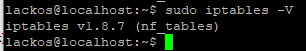
\includegraphics[scale=1.0]{images/iptables_nftables.png}
\caption{Debian 11-es rendszeren használt iptables, amely nftables backenddel dolgozik}
\end{figure}

Létezik iptables szabálylánc konvertáló program is, amelyre meglévő szabályainkat nftables syntaxra konvertálhatjuk. 

Az elkészített program az \texttt{iptables} backendet használja, mivel az a régebbi rendszereken is használható, továbbá még mindig elterjedt az \texttt{nftables} mellett is. Többféle elterjedt tűzfal implementáció is van, amelyek az \texttt{iptables}-t használják fel, a következő táblázatban kettőt fogok összehasonlítani.

\begin{table}[h]
\centering
\caption{ufw összehasonlítása firewalld-vel}
\label{tab:ispconfig}
\begin{tabularx}{\linewidth}{l|L|L}
 & ufw & firewalld \\
\hline
Használatának módja & CLI, de létezik hozzá GUI is & CLI, de létezik hozzá GUI is \\
\hline
Ingyenes & igen & igen \\
\hline
Parancsok formátuma & egyszerű parancsokkal rendelkezik, angol parancsok könnyű paraméterezéssel \cite{ufw} & kevésbé felhasználóbarát, komplexebb parancsok \cite{firewalld_man}\\
\hline
Támogatott protokollok & TCP, UDP. A ping engedélyezéséhez már iptables szabályokat kell írni & /etc/protocols-ból támogatja az összeset, portnál TCP/UDP/sctp/dccp protokollt támogat \\
\hline
Testreszabhatóság & nincsenek hozzá pluginok & nincsenek hozzá pluginok \\
\end{tabularx}
\end{table}

\pagebreak

\SubSection{OpenVPN}
A következő táblázatban a saját implementációmat, amely OpenVPN Community-t használ hasonlítom össze az OpenVPN Access Server-rel.

Fontos megemlíteni, hogy OpenVPN szerver menedzser implementáció több is létezik, létezik C\#-ban írt, létezik Bash Scriptben írt is. A minél nagyobb cross-platform támogatás lehetősége miatt azonban úgy gondolom mégis helyt áll a program létezése, a Lua nyelv egyszerűsége, nagyszerű cross-platform támogatása miatt. Értelemszerűen a Bash Script implementációk csak Linuxra korlátozódnak. GitHubon létezik web alapú interface is az OpenVPN Community Serverhez.

\begin{table}[h]
\label{tab:openvpn_apps}
\begin{tabularx}{\textwidth}{l|D|D}
 & OpenVPN Access Server \cite{openvpnaccessserver} & Saját implementáció (OpenVPN Community) \\
\hline
Ingyenes & nem & igen \\
\hline
Kliens támogatott OS & Cross-platform & Cross-platform \\
\hline
Szerver kezelés támogatott OS & a legtöbb támogatott & kizárólag Linux support\\
\hline
User authentikáció módja & webes alapú felhasználónév-jelszó, PAM, LDAP \newline RADIUS, SAML, stb. Saját auth script is készíthető. & kizárólag kulcs alapú (ez bővíthető saját auth scriptekkel, továbbá pluginokkal, például: PAM pluginnal). \\
\hline
Többfaktoros hitelesítés & beépített lehetőségek, továbbá pluginokkal bővíthető lehetőségek & saját auth scripttel kivitelezhető a 2FA, vagy akár pluginként \\
\hline
Access Control (ACL) & beépített lehetőségek & saját auth scripttel, vagy tűzfallal kivitelezhető \\
\hline
Tunnel átirányítás & beépített lehetőségek: full-tunnel és split-tunnel & megoldható a kliens konfigurálásával (a \texttt{route} program használatával) \\
\hline
Support & professzionális support ticketing rendszerrel & OpenVPN community fórum, Community Ticket report \\
\hline
Certificatek kezelése & automata, beépített tanusítványkezelés van, külső infrastruktúrát is lehet használni & saját, automatizált tanusítványkezelés \\
\hline
Kezelőfelület & webes alapú, command line & alapvetőleg command line, azonban webes alapú felület is lehetséges 3rd party szoftverekkel
\end{tabularx}
\end{table}
\Chapter{Tervezés}

A koncepciók, továbbá a felhasznált technológia kidolgozása után magára az alkalmazás tervezésére fordult a figyelmem. Elsőként kidolgoztam, hogy az alkalmazás kezelése hogyan menjen végbe, hogyan lehetne felhasználóbaráttá, ám mégis univerzálissá (a jövőbeli könnyebb fejlesztés jegyében) és könnyeddé alakítani az alkalmazást. Végül amellett döntöttem, hogy egy paranccsor alapú interaktív alkalmazást fogok létrehozni, amely paranccsori argumentumok nélkül fog működni.

\Section{Felhasználói felület, use-case diagram, use-case leírások}

Maga a tervezett felhasználói felület több menüpontból áll. Legelőször a főmenübe jutunk, ahonnan tudunk választani az alapfunkcionalitások közül, amelyeket már az előző, Koncepció című fejezetben megemlítettem. Ezek a szervereket jelentik, továbbá az iptables tűzfalat. Ezeken belül is többféle menüpontok találhatóak meg a kiválasztott funkcionalitásnak megfelelően. A menüpontok végén mindegyik almenü esetén szerepel a Visszalépés lehetőség. A navigálás egyszerűsítése érdekében minden egyes menüpontnak külön számot kell tartalmaznia. Menü váltáshoz az adott menüpont azonosító számát kell beírnunk, és ENTER-t kell nyomnunk. Néhány menüpont akár különböző adatokat is kérhet be, például weboldal létrehozásakor a weboldal címét, domainjét.
A program use-case diagramja \myaref{fig:usecase_diagram} ábrán található.

\begin{figure}[!h]
\centering
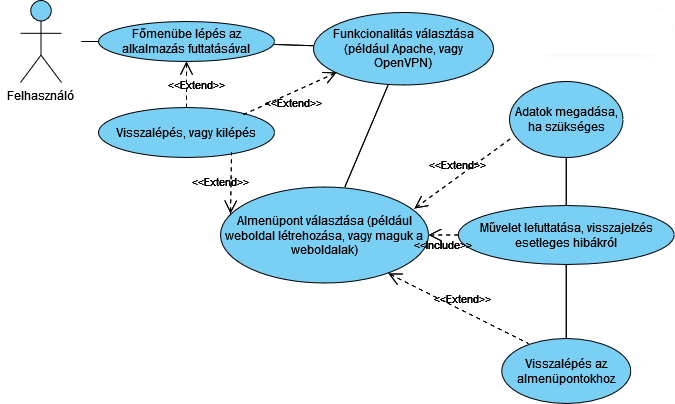
\includegraphics[scale=0.42]{images/usecase_diagram.png}
\caption{A program use-case diagramja}
\label{fig:usecase_diagram}
\end{figure}

\pagebreak

\SubSection{OpenVPN use-case leírása}

Az OpenVPN szerver konfigurálása közben a következőekben bemutatott esetek valósulhatnak meg. 

Ha nincs még feltelepítve az openvpn csomag, akkor fel kell telepítenünk azt. A csomag telepítése az \textit{apt-get} segédprogrammal megvalósítható, a csomag megléte pedig a \textit{dpkg-query} paranccsal ellenőrizhető, amellyel lekérhető egy adott csomag állapota megfelelő paraméterezéssel.

Feltelepítés után több dolgot is elő kell készíteni:
\begin{itemize}
	\item fel kell telepíteni az Easy-RSA-t, hogy saját tanusítványkezelőnk legyen mind a szerver mind a kliensek számára,
	\item létre kell hozni az Easy-RSA segítségével egy központi tanusítványt, továbbá a szervernek is egy tanusítványt és privát kulcsot,
	\item létre kell hozni az OpenVPN szervernek az \textit{\detokenize{/etc/openvpn}} adott aljegyzékében egy felhasználót \textit{\detokenize{/bin/false}} shellel a megnövelt biztonságért, amelyben futhat; ha már létezik ráfrissítünk, hogy biztos jó beállításai legyenek,
	\item létre kell hozni egy üres crl.pem fájlt, melybe később a visszavont kliensek tanusítványai kerülnek,
	\item generálni kell tls-auth fájlt az \textit{\detokenize{openvpn --genkey tls-auth}} parancs segítségével,
	\item be kell konfigurálni magát a szervert a \textit{server.conf}-ban: meg kell adni a létrehozott fájlok pathját az adott paraméterekhez (crl-verify, ca, cert, key, askpass, tls-crypt), meg kell adni a usert a server daemon számára (user, group), továbbá meg kell adni a chroot elérési útvonalát, amely a felhasználó home directoryja lesz,
	\item be kell állítani a \textit{\detokenize{/etc/default/openvpn}} fájlban az AUTOSTART értéket all-ra, és frissíteni kell a systemctl daemon-nal kapcsolatos beállításait a \textit{systemctl daemon-reload} paranccsal,
	\item be kell állítani a megfelelő jogosultságokat (chown és chmod) a fájlokon, jegyzékeken,
	\item ezek után pedig újra kell indítanunk a szervert.
\end{itemize}

Az előkészületek után lehet új kliens tanusítványt és privát kulcsot létrehozni, ezt a \textit{build-client-full} paraméterrel lehet megtenni az EasyRSA-ban. Célszerű jelszót használni a kulcs titkosításához. Ezután pedig egy minta konfiguráció módosításával tudjuk bekonfigurálni az új kliensünk konfigurációját, amelyet használhat az OpenVPN client segítségével. Ha valamely kliens hozzáférést vissza szeretnénk vonni, a \textit{revoke} EasyRSA paraméter van a segítségünkre. Ezután le kell futtatni a \textit{gen-crl} parancsot is, hogy tudja az OpenVPN szerver, mely kliens tanusítványok lettek visszavonva. A kliensek listája az EasyRSA mappájában az index.txt-ben található meg, ezt kell beolvasnunk ahhoz, hogy a jelenlegi kliensek listáját megkapjuk.

\SubSection{Apache use-case leírása}

Az Apache2 szerver adminisztrálása közben is több eset felmerülhet.

Legelőször is, ha még nincs feltelepítve az apache2 csomag, akkor azt fel kell telepítenünk. A feltelepítés és a csomag-ellenőrzés módszere megegyezik az OpenVPN esetében lévővel.

A csomag sikeres telepítése után az OpenVPN-hez képest valamivel kevesebb dolgot kell előkészítenünk:
\begin{itemize}
	\item létre kell hozni egy felhasználót \textit{\detokenize{/bin/false}} shellel, amelyben futhat maga az Apache2 daemon; ha ez már létezik, akkor beállításait frissíteni kell,
	\item létre kell hoznunk egy jegyzéket a weboldalak konfigurációinak tárolására (websiteconfigs), továbbá egy jegyzéket, ahol később a weboldalak tartalmai lesznek (wwwdatas),
	\item be kell állítani a megfelelő jogosultságokat (chown és chmod) a fájlokon, jegyzékeken,
	\item be kell konfigurálnunk a szervert úgy, hogy betöltse a saját weboldalunk konfigurációs fájljait (IncludeOptional beállítás); továbbá azt is be kell konfigurálnunk, hogy a wwwdatas jegyzéket elérhesse a daemon (Directory blokk létrehozása),
	\item be kell állítanunk az \textit{\detokenize{/etc/apache2/envvars}} fájlban az \detokenize{APACHE_RUN_USER, APACHE_RUN_GROUP} beállításokat, hogy a daemon az újonnan létrehozott felhasználót használja,
	\item ezek után újra kell indítanunk a szervert.
\end{itemize}
	
A megfelelő beállítások után már hozhatunk létre weboldalakat. Ehhez szükségünk lesz egy konfigurációs fájlra, amelyet a már előzőleg elkészített websiteconfigs jegyzékbe el kell helyezzünk. A konfigurációs fájlt egy megadott mintából kiindulva írjuk meg, kicserélve a megfelelő paramétereket (például ServerName, DocumentRoot). Ezután létre kell hoznunk a weboldalnak egy jegyzéket a wwwdatas jegyzéken belül, amelybe a weboldal tartalma kerül. A weboldalhoz létrehozunk egy index.html-t, amelybe egy üdvözlő üzenet kerül. Ezek után beállítjuk az újonnan létrehozott jegyzékek, fájlok jogosultságait, tulajdonosait. Weboldal törlésekor ki kell törölnünk az adott konfigurációs fájlt, a wwwdatas jegyzéken belül a weboldal jegyzékét, majd újra kell indítanunk a szervert.

SSL beállítása esetén először is meg kell győződnünk arról, hogy a headers és az ssl modul rendelkezésünkre áll, ezt a \textit{a2enmod headers} és \textit{a2enmod ssl} paranccsal tudjuk megtenni. Ezután megkeressük a Let's Encrypt által létrehozott minta SSL konfigurációt (amely frissítésre kerül általában automatikusan a megfelelő legújabb normáknak), és átmásoljuk egy megfelelő helyre. Miután sikeresen átmásoltuk, létrehozunk egy IfModule és VirtualHost blokkot (amely a 443-as portra mutat), amelyben el kell helyezni a már másik VirtualHost blokkban lévő beállításokat, továbbá ki kell egészíteni azt az SSL let's Encrypt fájl Include-olásával, paramétereivel (SSLCertificateFile, SSLCertificateKeyFile, SSLOpenSSLConfCmd, SSLCompression, Header).

\pagebreak

\SubSection{Nginx use-case leírása}

Az nginx szerver adminisztrálása hasonló lépéseket követel meg, mint az Apache2 szerver adminisztrálása.

Itt is a csomag telepítésével kezdünk, ha még nincs feltelepítve az nginx csomag. A feltelepítés és a csomag-ellenőrzés módszere megegyezik az OpenVPN esetében lévővel.

A csomag sikeres telepítése után szintén több dolgot szükséges előkészíteni:
\begin{itemize}
	\item létre kell hozni egy felhasználót \textit{\detokenize{/bin/false}} shellel, amelyben futhat maga az Apache2 daemon; ha ez már létezik, akkor beállításait frissíteni kell,
	\item létre kell hoznunk egy jegyzéket a weboldalak konfigurációinak tárolására (websiteconfigs), továbbá egy jegyzéket, ahol később a weboldalak tartalmai lesznek (wwwdatas),
	\item be kell állítani a megfelelő jogosultságokat (chown és chmod) a fájlokon, jegyzékeken,
	\item be kell konfigurálnunk a szervert úgy, hogy betöltse a saját weboldalunk konfigurációs fájljait (include beállítás), továbbá be kell állítanunk, hogy a daemon az újonnan létrehozott felhasználót használja (user paraméter).
\end{itemize}

A megfelelő beállítások után már hozhatunk létre weboldalakat. Ehhez szükségünk lesz egy konfigurációs fájlra, amelyet a már előzőleg elkészített websiteconfigs jegyzékbe el kell helyezzünk. A konfigurációs fájlt egy megadott mintából kiindulva írjuk meg, kicserélve a megfelelő paramétereket (például \detokenize{server_name, root}). Ezután létre kell hoznunk a weboldalnak egy jegyzéket a wwwdatas jegyzéken belül, amelybe a weboldal tartalma kerül. A weboldalhoz létrehozunk egy index.html-t, amelybe egy üdvözlő üzenet kerül. Ezek után beállítjuk az újonnan létrehozott jegyzékek, fájlok jogosultságait, tulajdonosait. Weboldal törlésekor ki kell törölnünk az adott konfigurációs fájlt, a wwwdatas jegyzéken belül a weboldal jegyzékét, majd újra kell indítanunk a szervert.

SSL beállítása esetén először megkeressük a Let's Encrypt által létrehozott minta SSL konfigurációt (amely frissítésre kerül általában automatikusan a megfelelő legújabb normáknak), és átmásoljuk egy megfelelő helyre. Miután sikeresen átmásoltuk, a már meglévő HTTP beállításokhoz a weboldal konfigurációjában beszúrjuk egy include beállítás segítségével. Ezután beállítjuk a megfelelő SSL paramétereket (\detokenize{add_header, ssl_dhparam, ssl_certificate, ssl_certificate_key, if ($scheme != "https") blokk, listen 443 ssl}), a már meglévő HTTP beállításokhoz való hozzáfűzéssel.

\SubSection{certbot use-case leírása}

Webszerverek üzemeltetése során szóba jöhet az SSL beállítása, ehhez lesz nekünk segítségül a certbot.

A certbot telepítése előtt a snapd csomagot szükséges telepítenünk az apt csomagkezelő segítségével, majd azt le kell frissíteni a \textit{snapd install --stable core} parancs segítségével. Ezután telepíthető a certbot a \textit{snapd install --stable --classic certbot} parancs segítségével. Hogy megtudjuk, már telepítve van-e a csomag, a \textit{snap list} parancs értelmezése van segítségünkre.

A csomag telepítése után létre kell hozni egy szimbolikus linket a \textit{ln -s /snap/bin/certbot /usr/bin/certbot} parancs segítségével, így tudjuk bárhonnan használni a certbot parancsot. SSL tanusítványok létrehozását kétféleképp is hozhatunk létre: HTTP-01 challenge és DNS-01 challenge segítségével. Mindkettőhöz külön parancs tartozik, a HTTP-01 challenge könnyebben automatizálható megfelelő paraméterekkel, a DNS-01-hez pedig szükséges egyedi authentikációs szkript létrehozása. Az SSL tanusítvány sikeres kiállítása után konfigurálnunk kell webszervereinket a már előzőleg megemlített módon. Célszerű dhparam fájlt is létrehozni, minél nagyobb bitszámmal, a megnövelt biztonság érdekében.

\SubSection{iptables use-case leírása}

Bármely szerver üzemeltetése során felmerül egy tűzfal beállítása, mint egy védelmi rendszer elemeként.

Az iptables használatához először meg kell győződnünk róla, hogy már fel van-e telepítve. Ha nincs, az apt csomagkezelő segítségével telepíteni tudjuk. Ezután beolvassuk és értelmezzük a már meglévő iptables szabályokat annak érdekében, hogy például tudjuk mely portok lehetnek nyitva, zárva. A jelenlegi iptables szabályokat a \textit{iptables-save} parancs segítségével tudjuk megnézni, ezt a fájlt szükséges értelmeznünk. A jelenlegi szabálykészletek felülírására a \textit{iptables-restore} parancsot használjuk.

Új portot az \textit{\detokenize{iptables -A INPUT -i interf}é\detokenize{sz -p protokoll --dport port --source }ipcím\detokenize{ -j ACCEPT}} parancs segítségével tudunk engedélyezni. Ebben a parancsban a source paraméter elhagyható. Ezt a szabályt célszerű legelőlre beszúrni.

Portot lezárni az \textit{\detokenize{iptables -A INPUT -i interf}é\detokenize{sz -p protokoll --dport port --source }ipcím\detokenize{ -j DROP}} parancs segítségével tudunk engedélyezni. Ebben a parancsban a source paraméter elhagyható. Ez a szabály bárhova beszúrható.

Új kimenő kapcsolatot az \textit{\detokenize{iptables -A OUTPUT -i interf}é\detokenize{sz -p protokoll --dport port --destination }ipcím\detokenize{ -j ACCEPT}} parancs segítségével tudunk engedélyezni. Ezt a szabályt célszerű legelőlre beszúrni. A protokoll és a port paraméter kihagyható.

Minden bejövő kapcsolatot, kivéve az engedélyezettet az \textit{\detokenize{iptables -A INPUT -i interf}é\detokenize{sz -j DROP}} paranccsal tudunk letiltani. Ezt a szabályt a szabályok levégére kell beszúrnunk.
Minden kimenő kapcsolatot, kivéve az engedélyezettet az \textit{\detokenize{iptables -A OUTPUT -i interf}é\detokenize{sz -j DROP}} paranccsal tudunk letiltani. Ezt a szabályt a szabályok levégére kell beszúrnunk.

Az előzőleg példaként adott parancsoknál az interfész paraméter mindenhol kihagyható (ekkor mindegyikre vonatkozni fog).

OpenVPN NAT-ot a következő parancsokkal tudunk engedélyezni:
\begin{itemize}
	\item \detokenize{iptables -A FORWARD -i IF_MAIN -o IF_TUNNEL -m state --state ESTABLISHED,RELATED -j ACCEPT}, ahol az \detokenize{IF_MAIN} a fő interfészünk, az \detokenize{IF_TUNNEL} pedig általában a tun0 interfész,
	\item \detokenize{iptables -A FORWARD -s YOUR_OPENVPN_SUBNET -o $IF_MAIN -j ACCEPT}, ahol az \detokenize{YOUR_OPENVPN_SUBNET} az OpenVPN szerverünk IP címét és subnetjét tartalmazza,
	\item \detokenize{iptables -t nat -A POSTROUTING -s YOUR_OPENVPN_SUBNET -o}\\\detokenize{IF_MAIN -j MASQUERADE}, ahol az \detokenize{YOUR_OPENVPN_SUBNET} az \\OpenVPN szerverünk IP címét és subnetjét tartalmazza, továbbá az \detokenize{IF_MAIN} a fő interfészt.
\end{itemize}

\pagebreak

A következő leírásokban, ábrákban bemutatom azokat a modulok struktúráját\\(UML diagramját), amelyek az előzőleg kifejtett use-casekat megvalósítják.

A program felépítése az OO alapelveket igyekszik követni. Elsősorban modulokból áll, amelyek osztályként is értelmezhetőek. Vannak olyan modulok, amelyekben csak a helyi scopeban elérhető kódok vagy változók vannak, tehát "private" elérésűek. Vannak olyan modulok, amelyekben több osztályok is találhatóak. A main modul (vagyis maga a main.lua) a felhasználói interfészt tartalmazza, ez használja fel a legtöbb modult.

A \myref{fig:visibilityrules} ábrán tekinthetőek meg a láthatósági szabályok az UML diagramokon.
\begin{figure}[h!]
	\centering
	\begin{tikzpicture}
		\begin {class}[text width=0.35\textwidth]{Láthatósági szabályok}{0, 0}
			\attribute {- Private}
			\attribute {+ Public}
		\end {class}
	\end {tikzpicture}
	\caption{Láthatósági szabályok az UML diagramokon}
	\label{fig:visibilityrules}
\end{figure}

\Section{general, apt\_packages, utils modulok felépítése, feladata}

Legelőször a \detokenize{general, linux, apt_packages} és az utils modul került megtervezésre. Felépítésük \myaref{fig:generalandaptpackages} ábrán látható.

\begin{figure}[h!]
	\centering
	\begin{tikzpicture}
		\begin {class}[text width=0.455\textwidth]{general}{0, 0}
			\attribute {+ \detokenize{lineEnding : string}}
			\operation {+ \detokenize{getOSType()}}
			\operation {+ \detokenize{clearScreen()}}
			\operation {+ \detokenize{sleep(n)}}
			\operation {+ \detokenize{strSplit(str, sep)}}
			\operation {+ \detokenize{deepCompare(tbl1, tbl2)}}
			\operation {+ \detokenize{concatPaths(...) -> varargs}}
			\operation {+ \detokenize{extractDirFromPath(path)}}
			\operation {+ \detokenize{readAllFileContents(filePath)}}
			\operation {+ \detokenize{trim2(s)}}
		\end {class}
		\begin {class}[text width=0.44\textwidth]{\detokenize{apt_packages}}{7.8, 0}
			\operation {+ \detokenize{isPackageInstalled(packageName)}}
			\operation {+ \detokenize{installPackage(packageName)}}
		\end {class}
	\end {tikzpicture}
	\caption{A general és \detokenize{apt_packages} modul felépítése}
	\label{fig:generalandaptpackages}
\end{figure}

A general modulban olyan funkciók és változók találhatóak, amelyek a legtöbb operációs rendszeren működnek, és fontos szerepet töltenek be a program működése közben.

Az \detokenize{apt_packages} modul Linux-specifikus kódokat tartalmaz, a modul feladata az apt program segítségével a csomagok menedzselése, telepítése.

Az utils modul legfőképp hibakeresésre volt használva, jelenleg épp nincs alkalmazva a program kódjában, így ezt a modult nem mutatom be.

\pagebreak

\Section{linux modul felépítése, feladatai}

A \myref{fig:linux_module} számú UML diagramon a linux nevezetű modult fogom bemutatni, amely linux-specifikus kódrészleteket tartalmaz. Erre a modulra épül a legtöbb modul.

\begin{figure}[h!]
\centering
	\begin{tikzpicture}%[scale=0.85, every node/.style={scale=0.85}]
		\begin {class}[text width=0.9\textwidth]{linux}{0, 0}
			\operation {+ \detokenize{exists(file)}}
			\operation {+ \detokenize{isDir(path)}}
			\operation {+ \detokenize{listDirFiles(path)}}
			\operation {+ \detokenize{mkDir(path)}}
			\operation {+ \detokenize{deleteFile(path))}}
			\operation {+ \detokenize{deleteDirectory(path)}}
			\operation {+ \detokenize{execCommand(cmd)}}
			\operation {+ \detokenize{getServiceStatus(serviceName)}}
			\operation {+ \detokenize{isServiceRunning(serviceName)}}
			\operation {+ \detokenize{isProcessRunning(name)}}
			\operation {+ \detokenize{stopService(serviceName)}}
			\operation {+ \detokenize{startService(serviceName)}}
			\operation {+ \detokenize{restartService(serviceName)}}
			\operation {+ \detokenize{systemctlDaemonReload()}}
			\operation {+ \detokenize{checkIfUserExists(userName)}}
			\operation {+ \detokenize{createUserWithName(userName, comment, shell, homeDir)}}
			\operation {+ \detokenize{updateUser(userName, comment, shell)}}
			\operation {+ \detokenize{getUserHomeDir(userName)}}
			\operation {+ \detokenize{execCommandWithProcRetCode(cmd, linesReturned, envVariables, redirectStdErrToStdIn)}}
			\operation {+ \detokenize{copy(from, to)}}
			\operation {+ \detokenize{copyAndChown(user, from, to)}}
			\operation {+ \detokenize{chown(path, userName, isDir)}}
			\operation {+ \detokenize{chmod(path, perm, isDir)}}
		\end {class}
	\end {tikzpicture}
	\caption{A linux modul felépítése}
	\label{fig:linux_module}
\end{figure}

A linux modul feladatai szerteágazóak:

\begin{itemize}
	\item vannak benne fájl- és könyvtár manipulációs funkciók,
	\item vannak benne parancsfuttató funkciók (amelyek közül az egyik tökéletesen kompatibilis Windows-sal is), továbbá servicet és systemctlt kezelő funkciók,
	\item vannak benne felhasználókat módosító funkciók (felhasználók létrehozása, módosítása, felhasználó létezésének ellenőrzése, felhasználó home dir lekérése),
	\item vannak benne fájl vagy jegyzék tulajdonost változtató funkciók,
	\item vannak benne fájl és jegyzék hozzáférési szabályokat változtató funkciók.
\end{itemize}

\Section{OpenVPN modulok felépítései, feladatai}

A következőekben az OpenVPN szerver kezelését kezdtem el megtervezni, implementálni. Az összes modul a program jegyzékén belül a \textbf{modules/vpnHandler} jegyzékben található meg.

Több részmodulra lett szétosztva:
\begin{itemize}
	\item \textbf{OpenVPN}: ez maga bootstrap modul, ebben van OpenVPN csomagot feltelepítő funkció, szervert indító/leállító funkció, továbbá ez a modul tölti be a \detokenize{server_impl} modult
	\item \textbf{\detokenize{server_impl}}: ez a modul kezeli a szerverrel kapcsolatos legtöbb dolgot:
	
	előkészíti a könyvtárakat, feltelepíti az Easy-RSA Certificate kezelőt, létrehoz egy saját tanusítványkezelőt (\textit{Certificate Authority}-t), szerver-oldali tanusítványokat és kulcsfájlokat generál, saját OpenVPN felhasználót hoz létre a szervernek, tls-auth/tls-crypt kulcsot generál, a szerver konfigurációt beüzemeli, beállítja a server daemon auto-startot a \textit{/etc/default/openvpn} fájlban

	\item \textbf{\detokenize{config_handler}}: az OpenVPN szerver és kliens konfigját kezelő modul, konfigurációs fájl beolvasást és írást valósít meg. A parser és writer az eredeti OpenVPN parser kódja alapján épült, amely megtalálható a \cite{openvpn_parser} hivatkozás alatt.
	\item \textbf{\detokenize{clienthandler_impl}}: ez a modul kezeli teljesen a klienssel kapcsolatos dolgokat:
	
	kliens tanusítványt, privát kulcsot hoz létre; kliens konfigurációt hoz létre, amelybe beleszúrja a generált fájlok tartalmát (így 1 db konfigurációs fájlra van szüksége az OpenVPN kliensnek); tanusítvány visszavonást támogat; továbbá le lehet kérni az összes jelenlegi klienst, amelyek valósak (nincsenek visszavonva)
\end{itemize}

Maga az OpenVPN bootstrap és \detokenize{config_handler} modul nagyon egyszerű felépítésű, amely látható is \myaref{fig:openvpn_module} és \myaref{fig:openvpn_config_handler_module} ábrán. 
\begin{figure}[h!]
\centering
	\begin{tikzpicture}[scale=0.83, every node/.style={scale=0.83}]
		\begin {class}[text width=0.7\textwidth]{OpenVPN}{0, 0}
			\attribute {+ \detokenize{errors : table}}
			\attribute {+ \detokenize{serverImpl -> }\textbf{OpenVPN\_server\_impl} module}
			\operation {+ \detokenize{isOpenVPNInstalled()}}
			\operation {+ \detokenize{installOpenvpn()}}
			\operation {+ \detokenize{isRunning()}}
			\operation {+ \detokenize{stopServer()}}
			\operation {+ \detokenize{startServer()}}
			\operation {+ \detokenize{initDirs()}}
		\end {class}
	\end {tikzpicture}
	\caption{Az OpenVPN bootstrap modul felépítése}
	\label{fig:openvpn_module}
\end{figure}

\begin{figure}[h!]
\centering
	\begin{tikzpicture}[scale=0.83, every node/.style={scale=0.83}]
		\begin {class}[text width=0.7\textwidth]{\detokenize{OpenVPN_config_handler}}{0, 0}
			\operation {+ \detokenize{parseOpenVPNConfig(linesInStr)}}
			\operation {+ \detokenize{writeOpenVPNConfig(parsedLines)}}
		\end {class}
	\end {tikzpicture}
	\caption{Az \detokenize{OpenVPN_config_handler} modul felépítése}
	\label{fig:openvpn_config_handler_module}
\end{figure}

A \detokenize{server_impl} modul minden OpenVPN szerverrel kapcsolatos művelet magja, ezért sok funkcióval rendelkezik. Felépítése \myaref{fig:openvpn_server_impl_module} ábrán látható. 

A klienseket kezelő \detokenize{OpenVPN_clienthandler_impl} modulban pedig két osztály is helyet foglal az OO alapelveket követve. Struktúrája \myaref{fig:openvpn_clienthandler_impl_module} ábrán látható.

\begin{figure}[h]
	\centering
	\begin{tikzpicture}[scale=0.84, every node/.style={scale=0.84}]
		\begin {class}[text width=1\textwidth]{\detokenize{OpenVPN_server_impl}}{0, 0}
			\attribute {- \detokenize{bootstrapModule -> }\textbf{\detokenize{OpenVPN}} module}
			\attribute {- \detokenize{caPass : string}}
			\attribute {- \detokenize{serverKeyPass : string}}
			\attribute {- \detokenize{sampleConfigFileContent : string}}
			\attribute {+ \detokenize{errors : table}}
			\operation {- \detokenize{registerNewError(errorName)}}
			\operation {- \detokenize{getConfigFilePath(openVPNConfigDir)}}
			\operation {+ \detokenize{constructor(_bootstrapModule)}}
			\operation {+ \detokenize{resolveErrorToStr(error)}}
			\operation {+ \detokenize{getEasyRSADir()}}
			\operation {+ \detokenize{getCAPass()}}
			\operation {+ \detokenize{getOpenVPNBaseConfigDir()}}
			\operation {+ \detokenize{isEasyRSAInstalled()}}
			\operation {+ \detokenize{formatPathInsideEasyRSAInstallCache(path)}}
			\operation {+ \detokenize{formatPathInsideBasedir(path)}}
			\operation {+ \detokenize{initDirs()}}
			\operation {+ \detokenize{installEasyRSA()}}
			\operation {+ \detokenize{getEasyRSAPKiDir()}}
			\operation {+ \detokenize{initEasyRSA()}}
			\operation {+ \detokenize{enableAllAutostartInDefault()}}
			\operation {+ \detokenize{getOpenVPNSubnet()}}
			\operation {+ \detokenize{checkServerConfig(homeDir, openVPNConfigDir)}}
			\operation {+ \detokenize{checkOpenVPNUserExistence()}}
			\operation {+ \detokenize{createOpenVPNUser(homeDir)}}
			\operation {+ \detokenize{updateExistingOpenVPNUser()}}
			\operation {+ \detokenize{getOpenVPNHomeDir()}}
			\operation {+ \detokenize{initializeServer()}}
		\end {class}
	\end {tikzpicture}
	\caption{Az \detokenize{OpenVPN_server_impl} modul felépítése}
	\label{fig:openvpn_server_impl_module}
\end{figure}

\begin{figure}[h!]
	\centering
	\begin{tikzpicture}[scale=0.84, every node/.style={scale=0.84}]
		\begin {class}[text width=0.458\textwidth]{\detokenize{OpenVPN_clienthandler_impl}}{0, 0}
			\attribute {- \detokenize{clientObjects : table}}
			\attribute {- \detokenize{validClients : table}}
			\attribute {- \detokenize{clientSampleConfig : string}}
			\attribute {+ \detokenize{errors : table}}
			\attribute {+ \textbf{Client}\detokenize{ -> class}}
			\operation {- \detokenize{getValidClientsFromPKIDatabase()}}
			\operation {- \detokenize{registerNewError(errorName)}}
			\operation {+ \detokenize{constructor(openVPNServerImpl)}}
			\operation {+ \detokenize{resolveErrorToStr(error)}}
			\operation {+ \detokenize{updateRevokeCRLForOpenVPNDaemon()}}
			\operation {+ \detokenize{getValidClients()}}
		\end {class}
		\begin {class}[text width=0.44\textwidth]{\detokenize{Client}}{8, 0}
			\attribute {- \detokenize{clientObjects : table}}
			\attribute {- \detokenize{validClients : table}}
			\attribute {- \detokenize{clientSampleConfig : string}}
			\attribute {+ \detokenize{errors : table}}
			\operation {+ \detokenize{new(clientName, loadedFromPKI)}}
			\operation {+ \detokenize{genKeyAndCRT(password)}}
			\operation {+ \detokenize{generateClientConfig()}}
			\operation {+ \detokenize{revoke()}}
			\operation {+ \detokenize{isValidClient()}}	
		\end {class}
		\unidirectionalAssociation{OpenVPN_clienthandler_impl}{}{}{Client}
	\end {tikzpicture}
	\caption{Az \detokenize{OpenVPN_clienthandler_impl} modul felépítése}
	\label{fig:openvpn_clienthandler_impl_module}
\end{figure}

\pagebreak

\Section{nginx modulok felépítései, feladatai}

Az nginx-et kezelő modulok is több részre lettek osztva. Az összes modul a program jegyzékén belül a \textbf{modules/nginxHandler} jegyzékben található meg. A modulok leírásai, feladatokkal:
\begin{itemize}
	\item \textbf{nginx}: ez maga egy bootstrap modul, ebben van nginx csomagot feltelepítő funkció, szervert leállító/elindító funkció, továbbá ez a modul tölti be a \\\detokenize{server_impl} modult.
	\item \textbf{\detokenize{server_impl}}: ez a modul kezeli a szerverrel kapcsolatos legtöbb dolgot:
	
	előkészíti a könyvtárakat, létrehoz az nginx daemonnak, workereknek egy felhasználót; támogatja automatikusan a weboldalak létrehozását, törlését; támogatja az SSL-t; minden támogatott funkciót bekonfigurál automatikusan.

	\item \textbf{\detokenize{config_handler}}: nginx szerver konfigurációját kezelő modul, beolvasást és írást implementál. A parser és writer az eredeti nginx parser kódja alapján épült, amely megtalálható a \cite{nginx_parser} hivatkozás alatt.
\end{itemize}

Az nginx bootstrap modul ezesetben is egyszerű felépítésű, amely látszik \myaref{fig:nginx_module} ábráról is. 

Azonban a \detokenize{config_handler} modul ebben az esetben már kissé bonyolultabb, mivel az nginx szintaxisa is komplikáltabb. Két osztályt tartalmaz. Struktúrája \myaref{fig:nginx_config_handler_module} ábrán látható.

\begin{figure}[h!]
	\centering
	\begin{tikzpicture}[scale=0.87, every node/.style={scale=0.87}]
		\begin {class}[text width=0.45\textwidth]{nginx}{0, 0}
			\attribute {+ \detokenize{errors : table}}
			\attribute {+ \detokenize{serverImpl -> }\textbf{nginx\_server\_impl} module}
			\operation {+ \detokenize{isInstalled()}}
			\operation {+ \detokenize{install()}}
			\operation {+ \detokenize{isRunning()}}
			\operation {+ \detokenize{stopServer()}}
			\operation {+ \detokenize{startServer()}}
			\operation {+ \detokenize{initDirs()}}
		\end {class}
	\end {tikzpicture}
	\caption{Az nginx bootstrap modul felépítése}
	\label{fig:nginx_module}
\end{figure}

\begin{figure}[h!]
	\centering
	\begin{tikzpicture}[scale=0.87, every node/.style={scale=0.87}]
		\begin {class}[text width=0.45\textwidth]{\detokenize{nginx_config_handler}}{0, 0}
			\attribute {+ \detokenize{nginxConfigHandler -> }\textbf{nginxConfigHandler} class}
			\operation {- \detokenize{concatArgsProperlyForBlockName(args)}}
			\operation {- \detokenize{parseNginxConfig(linesInStr)}}
			\operation {- \detokenize{formatDataAccordingQuoting(tbl)}}
			\operation {- \detokenize{doPaddingWithBlockDeepness(blockDeepness)}}
			\operation {- \detokenize{writeNginxConfig(parsedLines)}}
		\end {class}

		\begin {class}[text width=0.44\textwidth]{\detokenize{nginxConfigHandler}}{7.5, 0}
			\operation {+ \detokenize{new(linesInStr, paramToLine)}}
			\operation {+ \detokenize{getParsedLines()}}
			\operation {+ \detokenize{getParamsToIdx()}}
			\operation {+ \detokenize{insertNewData(dataTbl, pos)}}
			\operation {+ \detokenize{deleteData(pos)} - jelenleg nem használt}
			\operation {+ \detokenize{toString()}}
		\end {class}
		
		\unidirectionalAssociation{nginx_config_handler}{}{}{nginxConfigHandler}	
	\end {tikzpicture}
	\caption{Az \detokenize{nginx_config_handler} modul felépítése}
	\label{fig:nginx_config_handler_module}
\end{figure}

\pagebreak

A következő \myref{fig:nginx_server_impl_module} ábrán látható a \detokenize{nginx_server_impl} modul felépítése:

\begin{figure}[h!]
	\centering
	\begin{tikzpicture}[scale=0.90, every node/.style={scale=0.90}]
		\begin {class}[text width=0.7\textwidth]{\detokenize{nginx_server_impl}}{0, 0}
			\attribute {- \detokenize{sampleConfigForWebsite : string}}
			\attribute {+ \detokenize{nginxUser : string}}
			\attribute {+ \detokenize{nginxUserComment : string}}
			\attribute {+ \detokenize{nginxUserShell : string}}
			\attribute {+ \detokenize{baseDir : string}}
			\attribute {+ \detokenize{errors : table}}
			\operation {- \detokenize{registerNewError(errorName)}}
			\operation {+ \detokenize{constructor(_bootstrapModule)}}
			\operation {+ \detokenize{resolveErrorToStr(error)}}
			\operation {+ \detokenize{formatPathInsideBasedir(path)}}
			\operation {+ \detokenize{initDirs()}}
			\operation {+ \detokenize{checkNginxUserExistence()}}
			\operation {+ \detokenize{createNginxUser(homeDir)}}
			\operation {+ \detokenize{updateExistingNginxUser()}}
			\operation {+ \detokenize{getNginxHomeDir()}}
			\operation {+ \detokenize{getNginxMasterConfigPathFromDaemon()}}
			\operation {+ \detokenize{initializeServer()}}
			\operation {+ \detokenize{createNewWebsite(websiteUrl)}}
			\operation {+ \detokenize{deleteWebsite(websiteUrl)}}
			\operation {+ \detokenize{getCurrentAvailableWebsites()}}
			\operation {+ \detokenize{initSSLForWebsite(webUrl, certDetails)}}
		\end {class}
	\end {tikzpicture}
	\caption{Az \detokenize{nginx_server_impl} modul felépítése}
	\label{fig:nginx_server_impl_module}
\end{figure}

\Section{apache modulok felépítései, feladatai}

Az apache kezeléséhez tartozó modulok a program jegyzékén belül a \textbf{modules/apacheHandler} jegyzékben található meg.

A modulok leírásai, feladatokkal:
\begin{itemize}
	\item \textbf{apache}: ez maga egy bootstrap modul, ebben van apache2 csomagot feltelepítő funkció, szervert leállító/elindító funkció, továbbá ez a modul tölti be a \detokenize{server_impl} modult.
	\item \textbf{\detokenize{server_impl}}: ez a modul kezeli a szerverrel kapcsolatos legtöbb dolgot:
	
	előkészíti a könyvtárakat, létrehoz az Apache2 daemonnak, processeknek egy felhasználót\\támogatja automatikusan a weboldalak létrehozását, törlését; támogatja az SSL-t; minden támogatott funkciót bekonfigurál automatikusan (envvars fájl-t is).

	\item \textbf{\detokenize{config_handler}}: apache szerver konfigját kezelő modul:\\Konfiguráció írást és olvasást implementál. Az Apache2 szerver parsere az előzőleg tárgyalt programokhoz képest bonyolultabb, ezért teljesen az alapoktól terveztem ezt a modult. Ehhez maga a webszerver konfigurációjának szintaxis dokumentációját vettem segítségül, amely megtalálható a \cite{apache_configuring} hivatkozás alatt.
	\\Az envvars nevű fájl szerkesztését implementáló osztály is ebben a modulban van.
\end{itemize}

\pagebreak

Az Apache bootstrap modul ezesetben is egyszerű felépítésű, a \detokenize{config_handler} pedig három osztályt tartalmaz. A \detokenize{server_impl} modul hasonló bonyolultságú az \\\detokenize{nginx_server_impl} modulhoz. Felépítésük megtekinthető \myaref{fig:apache_modules} ábrán.
	
\begin{figure}[h!]
	\centering
	\begin{tikzpicture}[scale=0.95, every node/.style={scale=0.95}]
		\begin {class}[text width=0.45\textwidth]{apache}{0, 0}
			\attribute {+ \detokenize{errors : table}}
			\attribute {+ \detokenize{serverImpl -> }\textbf{apache\_server\_impl} module}
			\operation {+ \detokenize{isInstalled()}}
			\operation {+ \detokenize{install()}}
			\operation {+ \detokenize{isRunning()}}
			\operation {+ \detokenize{stopServer()}}
			\operation {+ \detokenize{startServer()}}
			\operation {+ \detokenize{initDirs()}}
		\end {class}
		
		\begin {class}[text width=0.45\textwidth]{\detokenize{apache_config_handler}}{7.6, 0}
			\attribute {+ \detokenize{apacheConfigHandler -> }\textbf{apacheConfigHandler} class}
			\attribute {+ \detokenize{apacheEnvvarsHandler -> }\textbf{apacheEnvvarsHandler} class}
			\operation {- \detokenize{parseApacheConfig(linesInStr)}}
			\operation {- \detokenize{doPaddingWithBlockDeepness(blockDeepness)}}
			\operation {- \detokenize{formatDataAccordingQuoting(tbl)}}
			\operation {- \detokenize{writeApacheConfig(parsedLines)}}
			\operation {- \detokenize{parse_envvar_args_from_line(line)}}
			\operation {- \detokenize{escapeMagic(s)}}
		\end {class}
		
		\begin {class}[text width=0.45\textwidth]{\detokenize{apacheConfigHandler}}{0, -6.5}
			\operation {+ \detokenize{new(linesInStr, paramToLine)}}
			\operation {+ \detokenize{getParsedLines()}}
			\operation {+ \detokenize{getParamsToIdx()}}
			\operation {+ \detokenize{insertNewData(dataTbl, pos)}}
			\operation {+ \detokenize{deleteData(pos)} - jelenleg nem használt}
			\operation {+ \detokenize{toString()}}
		\end {class}
		
		\begin {class}[text width=0.45\textwidth]{\detokenize{apacheEnvvarsHandler}}{7.6, -7}
			\operation {+ \detokenize{new(linesInStr)}}
			\operation {+ \detokenize{getArgs()}}
			\operation {+ \detokenize{toString()}}
		\end {class}
		
		\begin {class}[text width=0.45\textwidth]{\detokenize{apache_server_impl}}{7.6, -10.3}
			\attribute {+ \detokenize{apacheUser : string}}
			\attribute {+ \detokenize{apacheUserComment : string}}
			\attribute {+ \detokenize{apacheUserShell : string}}
			\attribute {+ \detokenize{baseDir : string}}
			\attribute {+ \detokenize{errors : table}}
			\attribute {- \detokenize{sampleConfigForWebsite : string}}
			\operation {- \detokenize{resolveErrorToStr(error)}}
			\operation {+ \detokenize{constructor(_bootstrapModule)}}
			\operation {+ \detokenize{formatPathInsideBasedir(path)}}
			\operation {+ \detokenize{checkApacheUserExistence()}}
			\operation {+ \detokenize{createApacheUser(homeDir)}}
			\operation {+ \detokenize{updateExistingApacheUser()}}
			\operation {+ \detokenize{getApacheHomeDir()}}
			\operation {+ \detokenize{getApacheMasterConfigPathFromDaemon()}}
			\operation {+ \detokenize{initDirs()}}
			\operation {+ \detokenize{initializeServer()}}
			\operation {+ \detokenize{createNewWebsite(websiteUrl)}}
			\operation {+ \detokenize{deleteWebsite(websiteUrl)}}
			\operation {+ \detokenize{getCurrentAvailableWebsites()}}
			\operation {+ \detokenize{initSSLForWebsite(webUrl, certDetails)}}
		\end {class}

		\unidirectionalAssociation{apache_config_handler}{}{}{apacheConfigHandler}
		\unidirectionalAssociation{apache_config_handler}{}{}{apacheEnvvarsHandler}
	\end {tikzpicture}
	\caption{Az apache implementáció moduljainak felépítése}
	\label{fig:apache_modules}
\end{figure}

\pagebreak

\Section{certbot modul felépítése, feladata}

A certbot csak egy modult foglal magában. Működéséhez több modult is felhasznál. A modulban megtalálható a certbot telepítése snapd-n keresztül, symlink létrehozás, SSL certificate létrehozás HTTP-01 challenge és DNS challenge segítségével, továbbá be is konfigurálja az adott webszervereket a használathoz.

Habár a certbot akár az \textit{apt} csomagkezelővel is feltelepíthető, az \textit{apt-get install certbot} parancs segítségével, maga a program weboldalán a leírás szerint snapd-vel telepítik. \cite{certbot_install_debian}

A különbség főképp a kettő között az, hogy az \textit{apt} csomagkezelő deb csomagokkal dolgozik, a \textit{snap} pedig teljes archívumokkal. Teljesen külön repository-kal dolgoznak.

Az apt esetében a függőségek külön rakódnak fel a csomagok feltelepítésekor, és a deb archívumok csak a csomagokat tartalmazzák. Ebben az esetben a frissítések késhetnek, mivel több szervezet, személy is átnézi a frissítés tartalmát.

A snapd esetében egy teljes archívumot tölt le a rendszer, ebben benne van a csomag összes függősége pont azzal a verzióval, amellyel a csomag fejlesztői szerették volna. Ez az archívum egy "zárt térbe" kerül kicsomagolásra, és limitált hozzáférése van magához a rendszerhez (hasonlóan a Docker-alkalmazásokhoz). Frissítéskor a fejlesztő adja ki a frissítéseket, nem validálják őket külön, ezáltal gyorsabban eljut a userekhez. \cite{snap_vs_apt}

A certbot modul UML diagramja \myaref{fig:certbot_module} ábrán látható.
	
\begin{figure}[h!]
	\centering
	\begin{tikzpicture}%[scale=0.95, every node/.style={scale=0.95}]
		\begin {class}[text width=0.6\textwidth]{\detokenize{certbot}}{0, 0}
			\attribute {- \detokenize{errors : table}}
			\attribute {- \detokenize{certFileName : string}}
			\attribute {- \detokenize{keyFileName : string}}
			\attribute {- \detokenize{dhParamFileName : string}}
			\attribute {- \detokenize{dryRunStr : string}}
			\attribute {- \detokenize{dhParamBytes : number}}
			\operation {- \detokenize{registerNewError(errorName)}}
			\operation {- \detokenize{sleep(n)}}
			\operation {+ \detokenize{resolveErrorToStr(error)}}
			\operation {+ \detokenize{isCertbotInstalled()}}
			\operation {+ \detokenize{createCertbotSymlink()}}
			\operation {+ \detokenize{installCertbot()}}
			\operation {+ \detokenize{getCertDatas(domain)}}
			\operation {+ \detokenize{trySSLCertificateCreation(method, domain, webserverType)}}
			\operation {+ \detokenize{init()}}
		\end {class}
	\end {tikzpicture}
	\caption{A certbot modul felépítése}
	\label{fig:certbot_module}
\end{figure}

A \textit{dryRunStr} és a \textit{dhParamBytes} változó kitüntetett figyelmet érdemel. 

A dryRunStr változó csak hibakereséskor használatos, debug esetén a \detokenize{--dry-run} paramétert lehet beleírni. Ezzel célszerű lehet a certbot működését tesztelni, kifejezetten arra van kitalálva, ilyenkor nem valódi SSL tanusítvány generálódik, továbbá az API limitációja sem olyan szigorú.

A dhParamBytes változó pedig a program jelenlegi kódjában megkönnyítve a tesztelést 1024 bitre van állítva, azonban célszerű megnövelni a bitszámot akár magasabb értékekre is, például 2048. Ez lelassítja az SSL tanusítványok beállításának folyamatát.

\Section{iptables modul felépítése, feladata}

Ez a modul kezeli a tűzfalszabályokat az \textit{iptables} frontend segítségével. Funkcionalitása maga az iptables telepítése, a portok nyitása/zárása, kimenő/bemenő csomagok szűrése, a már meglévő beállítások lekérdezésének implementálása, továbbá a NAT előkészítése az OpenVPN szerver számára. 

A modul UML diagramja \myaref{fig:iptables_module} ábrán tekinthető meg:

\begin{figure}[h!]
	\centering
	\begin{tikzpicture}%[scale=0.9, every node/.style={scale=0.9}]
		\begin {class}[text width=0.9\textwidth]{\detokenize{iptables}}{0, 0}
			\attribute {- \detokenize{iptablesAliases : table}}
			\attribute {+ \detokenize{errors : table}}
			\operation {+ \detokenize{resolveErrorToStr(error)}}
			\operation {+ \detokenize{isIptablesInstalled()}}
			\operation {+ \detokenize{installIptables()}}
			\operation {+ \detokenize{getCurrentNetworkInterfaces()}}
			\operation {+ \detokenize{getCurrentSSHPorts()}}
			\operation {+ \detokenize{parseCurrentRules()}}
			\operation {+ \detokenize{getOpenPorts(interface)}}
			\operation {+ \detokenize{deleteOpenPortRule(interface, idx)}}
			\operation {+ \detokenize{getClosedPorts(interface)}}
			\operation {+ \detokenize{deleteClosePortRule(interface, idx)}}
			\operation {+ \detokenize{closePort(interface, protocol, dport, fromIP)}}
			\operation {+ \detokenize{openPort(interface, protocol, dport, fromIP)}}
			\operation {+ \detokenize{listAllowedOutgoingConnections(interface)}}
			\operation {+ \detokenize{deleteOutgoingRule(interface, idx)}}
			\operation {+ \detokenize{allowOutgoingNewConnection(interface, protocol, dip, dport)}}
			\operation {+ \detokenize{checkIfInboundPacketsAreBeingFilteredAlready(interface, protocol)}}
			\operation {+ \detokenize{togOnlyAllowAcceptedPacketsInbound(toggle, interface, protocol)}}
			\operation {+ \detokenize{checkIfOutboundPacketsAreBeingFilteredAlready(interface, protocol)}}
			\operation {+ \detokenize{togOnlyAllowAcceptedPacketsOutbound(toggle, interface, protocol)}}
			\operation {+ \detokenize{deleteNATRules(mainInterface, tunnelInterface, forwardTblIdx, forwardTblAllIdx, postroutingTblAllIdx)}}
			\operation {+ \detokenize{getCurrentActiveNATForOpenVPN()}}
			\operation {+ \detokenize{initNATForOpenVPN(mainInterface, tunnelInterface, openvpnSubnet)}}
			\operation {+ \detokenize{loadOurRulesToIptables()}}
			\operation {+ \detokenize{iptablesToString()}}
			\operation {+ \detokenize{initModule()}}
		\end {class}
	\end {tikzpicture}
	\caption{Az iptables modul felépítése}
	\label{fig:iptables_module}
\end{figure}

\Section{snapd modul felépítése, feladata}

A snapd modul egyszerű felépítésű. Feladata maga a snapd feltelepítése az \textit{apt} csomagkezelő segítségével, továbbá csomagok telepítése, és a már feltelepített csomagok meglétének ellenőrzése.

A snapd modul UML diagramja a következő \myref{fig:snapd_module} ábrán található meg.
	
\begin{figure}[!h]
	\centering
	\begin{tikzpicture}%[scale=0.95, every node/.style={scale=0.95}]
		\begin {class}[text width=0.6\textwidth]{\detokenize{snapd}}{0, 0}
			\operation {+ \detokenize{isSnapdInstalled()}}
			\operation {+ \detokenize{installSnapd()}}
			\operation {+ \detokenize{isPackageInstalled(packageName)}}
			\operation {+ \detokenize{installPackage(packageName, classic)}}
		\end {class}
	\end {tikzpicture}
	\caption{A snapd modul felépítése}
	\label{fig:snapd_module}
\end{figure}
\Chapter{Megvalósítás}

A megvalósítás a már előző fejezetben tervezett struktúrát követte. Ebben a fejezetben néhány modul érdekesebb részeit fogom bemutatni, amelyek implementáció szempontjából nem biztos, hogy triviálisak.

\Section{linux modul érdekességei}

A legelsők közt készült el a \textit{linux} modul megvalósítása, mivel több modul is függött a funkcionalitásától. Néhány érdekesebb részt szeretnék bemutatni, mint például az \texttt{exists}, \texttt{isdir} implementációját:

\begin{lua}
function module.exists(file)
    local ok, err, code = os.rename(file, file)
    if not ok then
		return code == 13 or code == 17
    end
    return ok, err
end
function module.isDir(path)
    return module.exists(path.."/")
end
\end{lua}

Ez a kód úgy nézi meg a fájlok létezését, hogy megpróbálja a fájlokat átnevezni saját magukra. Ekkor kétféle error lehetséges: \textbf{Permission Denied} (code 13) vagy \textbf{File exists} (code 17). Jegyzékek létezését pedig úgy ellenőrzi, hogy hozzárakja a path végéhez a \textit{/} jelet, mivel így biztos, hogy jegyzékre mutat a path.

Érdekes lehet még az \texttt{\detokenize{execCommand}} és a \texttt{\detokenize{execCommandWithProcRetCode}} funkció implementációja is. Ezek a funkciók a program gerincét képezik, a legtöbb modul használja őket.

\begin{lua}
function module.execCommand(cmd)
    local handle = io.popen(cmd);
    local result = handle:read("*a");
    handle:close();
    return result;
end
\end{lua}

Az \texttt{\detokenize{execCommand}} egyszerű implementációjú, amely az \textit{io} standard library popen funkcióját használja meg egy processz megnyitására. Ez egy handlet ad. A read megvárja míg lefut a processz, majd az \textit{\detokenize{*a}} paraméter segítségével mindent kiolvas a pipeból. A végén lezáródik a handle. Windows rendszeren is tökéletesen működik.

A következő funkció az \texttt{\detokenize{execCommandWithProcRetCode}}. Itt a forráskódból kivettem az üres sorokat a kompaktabb kód érdekében. Működése nagyban hasonlít az \texttt{\detokenize{execCommand}}-hoz, azzal a kivétellel, hogy ez az implementáció felhasznál bizonyos Bash-script elemeket. Például az \textit{export} funkciót az environment variablek beállítására, vagy a \textit{\detokenize{$?}} változót a process return kód lekérésére. Támogatja az stderr átirányítását is stdout-ba (ez a \texttt{\detokenize{2>&1}} paraméter) cross-platform módon, a többi Bash alapú megoldás kivételével. A return code-t az utolsó sorba iratja ki, ezt olvassa be magától, és vágja ki az alap program outputjából.
\begin{lua}
function module.execCommandWithProcRetCode(cmd, linesReturned, envVariables, redirectStdErrToStdIn)
    local exportCmd = "";
    if envVariables then
        for k, v in pairs(envVariables) do
            exportCmd = exportCmd.." export "..tostring(k).."="..tostring(v).."; ";
        end
    end
    local handle = io.popen(exportCmd..cmd..tostring(redirectStdErrToStdIn and " 2>&1" or "").."; echo $?");
    handle:flush();
    local overallReturn = "";
    local lastLine = "";
    local newLineChar = "\n";
    local lineNum = 0;
    for line in handle:lines() do
        overallReturn = overallReturn .. line .. newLineChar;
        lastLine = line;
        lineNum = lineNum + 1;
    end
    handle:close();
    local retCode = tonumber(lastLine);
    if lineNum == 1 then
        overallReturn = "";
    else
        overallReturn = string.sub(overallReturn, 1, #overallReturn - #lastLine - #newLineChar * 2); --skip return code line
    end
    if linesReturned then
        return overallReturn, retCode;
    end
    return retCode;
end
\end{lua}

\pagebreak
\SSubSection{Processzek visszatérési értékeinek felhasználása}{Processzek visszatérési értékei}
Valamennyi funkció a programban kihasználja azt, hogy a processzek egy meghatározott visszatérési értéket (pontosabban \textit{exit code}-t) adnak vissza lefutásuk után. Ezeknek jelentőségük van, mivel bizonyos műveleteknél más értékeket adhatnak vissza attól függően, hogy milyen funkcionalitást használunk épp. Találhatunk olyan listát az Interneten, amelyek ezeket a kódokat általánosságban írják le, hogy milyen hibához kapcsolódhatnak. 
Általában a processzek visszatérési értékeinek jelentése valamennyire hasonlít a legtöbb táblázatban hozzákapcsolt leíráshoz. \cite{linux_exitcodes}

A legfontosabb, hogy általában a legtöbb processz \textit{0}-s értékkel fog visszatérni, ha sikeresen lezajlott a a processz futása, hiba nélkül. Ezt több programrész is felhasználja, például:

\begin{lua}
function module.checkIfUserExists(userName)
    local retCodeForId = module.execCommandWithProcRetCode("id "..userName);
    return retCodeForId == 0;
end
\end{lua}

Ebben az esetben a \texttt{\detokenize{checkIfUserExists}} funkció az alapján tudja egy felhasználó létezését, hogy \textit{0}-s exit code-val tért-e vissza az \textit{id} processz.

Vagy másik példaként az \textit{mkdir} parancs \textit{0}-s (néhány táblázat szerint: \textbf{Success}) visszatérési értékkel tér vissza akkor, ha sikerült létrehozni egy új jegyzéket, vagy \textit{1}-es (néhány táblázat szerint: \textbf{Operation not permitted}) visszatérési értékkel tér vissza akkor, ha már létezik az a jegyzék, amit létre szeretnénk hozni. A programkód is ez alapján dönti el, hogy sikeres-e a jegyzék létrehozása:
\begin{lua}
function module.mkDir(path)
    local retCodeForMkdir = module.execCommandWithProcRetCode("mkdir "..path);
    return retCodeForMkdir == 0 or retCodeForMkdir == 1; --new dir successfully created/already exists
end
\end{lua}

Ez szintén hasonlóan működhet olyan programoknál is, amelyek nem rendszerprogramok, hanem valaki más készítette őket. Például a \textit{certbot} is különböző processz visszatérési értékkel térhet vissza az adott művelet sikerességétől függően:
\begin{lua}
function module.trySSLCertificateCreation(method, domain, webserverType)
    ...
    local retLines, retCode = linux.execCommandWithProcRetCode("certbot certonly -n "..tostring(dryRunStr).." --agree-tos --no-eff-email --email \"\" --webroot --webroot-path "..tostring(websiteData.rootPath).." -d "..tostring(domain), true, nil, true);
    ...
    local hasCertificate = retCode == 0;
    ...
end
\end{lua}

\pagebreak
\Section{Háttérben futó processz eredményeire való várás}

A program tervezése, implementálása során belefutottam egy nehézségbe, amely a Lua alapvető kialakításából fakad: a Lua alapvetően egy szálon fut, és nem eseményalapú felépítésű. Létezik \textit{coroutine} beépített library, azonban az \textit{könnyű szál} alapú implementáció. Egyszerre csak egy coroutine futhat, és maga a coroutine kezdeményezheti azt, hogy épp felfüggesztve, suspendelve legyen (tehát visszaadja az irányítást az őt futtató kódnak, vagy más coroutinenak). Emiatt a coroutine sem volt megoldás erre a nehézségre.

A \textit{certbot} modul tervezése, implementálása közben jött elő ez a nehézség. A \textit{HTTP-01} challenget könnyen lehetett implementálni úgy, hogy megvártuk az újonnan létrehozott processz futási eredményeit, mivel az támogatta a nem-interaktív módot. Azonban a \textit{DNS-01} challenget nem lehet ilyen könnyen implementálni.

A probléma ott kezdődött, hogy a \textit{certbot} maga alapvetőleg sajnos nem támogatja azt, hogy nem-interaktív módon fut ezen challenge esetében. Megoldást azonban az jelentett, hogy \textit{\detokenize{--manual}} módban használjuk, és megadjuk neki a preferált challenget (vagyis a dns-t), továbbá \textit{manual-auth-hook} scriptet használunk. 

Ezzel a probléma felét már sikerült orvosolnunk, azonban előjött egy újabb probléma: az io.popen esetén a program megvárja a processz futásának végét. Ez azonban nekünk nem megfelelő, mivel akkor teljesen befagy a program, a DNS challenge futtatásakor pedig a felhasználónak meg kell jelenítenünk bizonyos adatokat, hogy milyen DNS rekordokat hozzanak létre a saját domainjükön és milyen értékekkel. Az \textit{os} függvénykönyvtárban található \texttt{execute} funkció másképp működik, hátránya, hogy alapvetően ez is blocking funkció, továbbá nem is tudjuk pontosan, hogy sikerült-e a program elindítása, csak akkor, ha van visszatérési értéke és megvizsgáljuk azt.
Ezután azzal folytattam a probléma megoldását, hogy Bash szkript elemeket használtam fel a program futtatásához, például a \texttt{\detokenize{&}} szimbólumot a háttérben való futáshoz, \textit{\detokenize{$?}} szimbólumot a státusz kód megkapásához, továbbá \textit{\detokenize{$!}} szimbólumot az újonnan elindított program folyamatazonosítójának megkapásához. Ezt az egészet egy nagy parancsba foglaltam. A parancs több fájlt is felhasznál:
\begin{itemize}
    \item Egy ideiglenes fájlt abból célból, hogy az újonnan létrehozott processz, továbbá a mostani processz kommunikálni tudjon egymással. Amint lefutott a certbot, ide kerül mentésre a visszatérési értéke,
    \item Egy másik ideiglenes fájlt abból a célból, hogy az újonnan létrehozott processz stdoutját és stderr pipeját abba irányítjuk, így a mostani processz tudja a kimenetet vizsgálni,
    \item Egy certbot\_pid.txt fájlt, amelyből tudjuk, hogy sikeresen lefutott-e a programunk. Azt a célt is szolgálja, hogy ha esetleg megszakadt a program futása valami miatt, akkor a következő lefutáskor a kill parancs segítségével megszüntessük a már nem használt processzt.
\end{itemize}

A kommunikáció maga a két processz között úgy történik, hogy elindul az auth Lua szkript a certbotban, amely megkapja környezeti változókon keresztül a certbottól az adatokat. Ezeket az adatokat a legelsőnek létrehozott ideiglenes fájlba írja bele, majd ezután 1 másodpercenként folyamatosan kiolvassa a tartalmát. Ez azért fontos, mert addig is blokkolja a certbot processzt, így nem halad tovább.\\Amint a felhasználó késznek nyilvánította a DNS rekordot, akkor ebbe az ideiglenes fájlba beleírodik a "ready" szó, majd ezután fut le csak a certbot DNS challengeje (megszakad a while true ciklus).

A Lua kódból néhány részletet kiemelve így néz ki az implementáció:
\begin{lua}
function module.trySSLCertificateCreation(method, domain, webserverType)
    ...
    local tempFileName = os.tmpname();
    local tempFileNameForStdOut = os.tmpname();

    local certbotPIDStuff = general.readAllFileContents("certbot_pid.txt");

    if certbotPIDStuff then
        os.execute("kill -9 "..tostring(certbotPIDStuff));
    end

    linux.deleteFile("certbot_pid.txt");

    local formattedCmd = "(certbot certonly -n "..tostring(dryRunStr).." --agree-tos --no-eff-email --email \"\" --manual --preferred-challenges dns --manual-auth-hook \"sh ./authenticator.sh \""..tostring(tempFileName).."\"\" -d "..tostring(domain).." > \""..tostring(tempFileNameForStdOut).."\" 2>&1; echo $? > \""..tostring(tempFileName).."\") & echo $! > certbot_pid.txt";
    os.execute(formattedCmd);

    if not linux.exists("certbot_pid.txt") then
        return module.EXEC_FAILED;
    end
    ...
    --fajlolvasas, cleanup
    ...
end
\end{lua}

Authentikátor szkript részlet:
\begin{lua}
while true do
    local fileHandle = io.open(fileName, "r");
    if fileHandle then
        local readStr = fileHandle:read("*a");
        fileHandle:close();
        if readStr:find("ready", 0, true) == 1 then
            break;
        end
    end
    sleep(1);
end
\end{lua}
\pagebreak
\Section{Konfigurációs fájlok módosításának implementációja}

A konfigurációs fájlok módosításához többféle modul is implementálva lett, ezeket a Tervezés című fejezetben meg is említettem: \textit{\detokenize{apache_config_handler}},\\\textit{\detokenize{nginx_config_handler}} és \textit{\detokenize{OpenVPN_config_handler}}. Ezek közül a modulok közül a legtöbb OO alapelveket igyekezett követni, az OpenVPN config handler kivételével.

A konfiguráció író és olvasó modulokat hasonlóképp ugyanarra a kódbázisra építettem fel, ez az Apache szerver \textit{envvars} fájl kezelőjének kivételével sikerült is. Mindegyik beolvasás kimenete általában két nagyobb táblából épül fel: \textit{\detokenize{parsedLines}} és \textit{\detokenize{paramToLine}}.
A \textit{parsedLines} maga az állapot tábla, abba van benne minden egyes beolvasott és értelmezett sor, benne paraméterek, kommentek vannak. A \textit{paramToLine} tábla általában csak gyorsítótár, azt mutatja meg, hogy bizonyos paraméterek hol vannak elhelyezkedve a parsedLines táblán belül, így nem kell átfésülni az egész parsedLines táblát egy adott paraméter keresésekor.

\SubSection{OpenVPN config parser-writer implementáció felépítése, használata}
A \textit{parsedLines} felépítése OpenVPN esetén egyszerű tömb, minden tömb elem egy tábla, amelyben a következő paraméterek szerepelhetnek:

\begin{itemize}
    \item \textbf{params}: Ez tartalmazza az adott paramétereket, opciókat egy adott sorban. A táblában található \textit{val} érték maga a paraméter értéke (vagy akár a konfigurációs beállítás neve), a \textit{state} pedig kifejezi az idézőjeltípust, ha használnak (ami lehet \textit{reading\_quoted\_param} \detokenize{"} esetén, vagy \textit{reading\_squoted\_param} \detokenize{'} esetén),
    \item \textbf{comment}: Ez tartalmazza az adott sorban található kommentet. Ha a \textit{params} tábla nem létezik, akkor maga az egész sor egy komment sor, ha létezik, akkor pedig a paraméterek után van a komment elhelyezve. Üres sor, ha ez sem létezik.
\end{itemize}

Kódrészlet OpenVPN szerver konfiguráció összeállítására a programból:

\begin{lua}
function module.checkServerConfig(homeDir, openVPNConfigDir)
...
    local configFileContent, paramsToLines = config_handler.parseOpenVPNConfig(sampleConfigFileContent);
    if paramsToLines["user"] then
        local paramTbl = configFileContent[paramsToLines["user"]];
        paramTbl["params"][2].val = module["openvpn_user"];
    end
...
    configFileHandle:write(config_handler.writeOpenVPNConfig(configFileContent));
    configFileHandle:flush();
    configFileHandle:close();
...
end
\end{lua}
\pagebreak

Az előző oldalon látható kódrészlet egy teljesen új konfigurációs fájlt generál az OpenVPN szerver számára. Ezt úgy teszi meg, hogy egy előre megadott alap konfigurációt beolvas, majd azon módosítja a paramétereket (például az user beállítást), utána pedig rendes konfigurációs szöveggé alakítja a módosított konfigurációt az állapot táblából. Az átírt argumentum \myaref{fig:openvpn_config_edit_example} ábrán látható.

\begin{figure}[h]
\centering
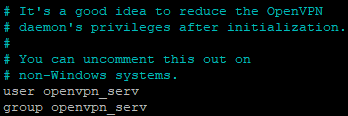
\includegraphics[scale=1.0]{images/openvpn_config_edit_example.png}
\caption{Az átírt \detokenize{user} argumentum. A példa konfigurációban nobody van használva}
\label{fig:openvpn_config_edit_example}
\end{figure}

\SubSection{Apache, nginx config parser-writer implementáció}

Az \textit{\detokenize{apache_config_handler}}, és az \textit{\detokenize{nginx_config_handler}} modulok már OO alapelveket követnek, azonban itt is fontos a két tábla felépítése. Az OpenVPN szerverhez képest a két szerver konfigurációs fájljai bonyolultabb és kiterjedtebb szintaxisú. Bár a konfigurációs fájl értelmező és író ugyanúgy két táblával dolgozik, megfigyelhető, hogy sokkal több paramétert tartalmaz egy adott sort leíró tábla.

A \textit{parsedLines} felépítése Apache és nginx esetén szintén egyszerű array, minden array elem egy tábla (és egy sor), amelyben a következő paraméterek szerepelhetnek (akár több is egyszerre):

\begin{itemize}
    \item \textbf{spacer}: Üres sort jelent. Ha ez létezik, akkor a többi lentebb sorolt paraméter biztosan nem létezik az adott elemtáblában,
    \item \textbf{blockStart}: Egy blokk kezdetét jelenti, a blokk azonosítóját tartalmazza. Apache esetében argumentumok is tartozhatnak hozzá (tehát ilyenkor az args paraméter is feldolgozódik),
    \item \textbf{blockEnd}: Egy blokk végét jelenti, a lezárandó blokk azonosítóját tartalmazza,
    \item \textbf{paramName}: Adott sorban található beállítás nevét tartalmazza (például nginx esetében include, Apache esetében ServerName), egy táblában, amely ugyan úgy épül fel, mint az args paraméter. Természetesen mellé feldolgozódik az args paraméter is.
    \item \textbf{comment}: Ez tartalmazza az adott sorban található kommentet. Ha az \textit{args} tábla nem létezik, akkor maga az egész sor egy komment sor, ha létezik, akkor pedig a paraméterek után van a komment elhelyezve nginx esetén. Az Apache nem támogat kommenteket a sorok végén, az optionok és argumentumok után,
    \item \textbf{blockDeepness}: Megadja, hogy az adott sor mennyire van eltolva indent-ügyileg,
    \item \textbf{args}: több elem esetében is használatos paraméter (például Apache esetében blockStartnál is, paramName-nél pedig mindkettő implementációnál), amely egy tábla, és az adott művelethez tartalmaz paramétereket:
        \begin{itemize}
            \item \textbf{quoteStatus}: lehet \textit{d}, ekkor duplaidézőjelben van a paraméter; lehet \textit{s}, ekkor két sima idézőjel között van a paraméter,
            \item \textbf{multipleLine}: Apache esetében használatos, ha egy paraméter több sort is magába ölel (Apache-ban támogatott a több sor a \texttt{\detokenize{\\}} jelölés segítségével),
            \item \textbf{data}: ez maga egy szöveg, amely a paraméterhez tartozó adatokat tartalmazza.
        \end{itemize}
\end{itemize}

A két modul használata valamelyest eltér az előző OpenVPN konfigurációt kezelő modultól. Ezek már OO alapelveket követnek, továbbá valamennyivel több funkciót is implementálnak, szélesebb körben vannak használva a programban. Például van implementálva funkció arra, hogy teljesen új adatot tudjunk beszúrni bárhova, erre az OpenVPN szerver kezelő implementációja közben nem volt szükség.

A következőekben két rövid kódrészletet fogok mutatni Apache és nginx esetében is a modulok használatáról. Nginx esetében a következőképp kerül beállításra az SSL egyik beállítása:
\begin{lua}
function module.initSSLForWebsite(webUrl, certDetails)
    ...
    --Redirect unencrypted connections
    local blockName = 'if ($scheme != "https")';
    local blockStartSchemeIdx = paramsToIdx["block:"..tostring(blockName)];
    if not blockStartSchemeIdx then
    local blockDeepness = serverNameData.blockDeepness;
        configInstance:insertNewData({["comment"] = " Redirect unencrypted connections", blockDeepness = serverNameData.blockDeepness}, posStart);
        posStart = posStart + 1;
        configInstance:insertNewData({["blockStart"] = blockName, block = serverNameData.block, blockDeepness = serverNameData.blockDeepness, args = {}}, posStart);
        posStart = posStart + 1;
        blockDeepness = blockDeepness + 1;
        configInstance:insertNewData({["paramName"] = {data = 'rewrite'}, block = blockName, blockDeepness = blockDeepness, args = {{data = "^"}, {data = "https://$host$request_uri?"}, {data = "permanent"}}}, posStart);
        posStart = posStart + 1;
        blockDeepness = blockDeepness - 1;
        configInstance:insertNewData({["blockEnd"] = blockName, block = serverNameData.block, blockDeepness = serverNameData.blockDeepness, args = {}}, posStart);
        posStart = posStart + 1;
    end
    ...
end
\end{lua}
A kódrészlet megkeresi a \detokenize{'if ($scheme != "https")'} blokkot az adott weboldal nginx-konfigurációjában. Ha nem találja meg beszúr egy kommentet, majd azután beszúr egy blokk-kezdést. A blokkba beilleszti a \detokenize{'rewrite ^ https://$host$request_uri? permanent'} parancsot, majd lezárja a blokkot a parancs után. Mindezeket indentálva teszi, így a konfiguráció jól átlátható marad. A beállítás maga azt jelenti, hogy minden HTTP-n keresztüli csatlakozást átirányít HTTPS-re.

A gyakorlatban \myaref{fig:inserted_block_nginx} ábrán látható módon néz ki a beillesztett blokk, az nginx konfigurációjában.
\begin{figure}[h]
\centering
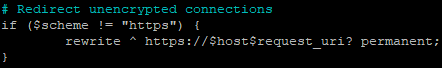
\includegraphics[scale=1.0]{images/nginx_config_edit_example.png}
\caption{A beillesztett blokk}
\label{fig:inserted_block_nginx}
\end{figure}

Apache esetében is hasonlóan működik a konfiguráció módosítása. Ott azonban teljesen külön blokkot kell csinálni az SSL konfigurációnak, teljesen új beállításokkal, továbbá a jelenlegi beállítások hozzáfűzésével, ezért az azt beállító kódrészlet hosszabb az nginx-implementációtól. Rövid kódrészlet az Apache SSL beállításából:
\begin{lua}
function module.initSSLForWebsite(webUrl, certDetails)
    ...
    blockDeepness = blockDeepness + 1;
    configInstance:insertNewData({
        blockStart = "VirtualHost",
        args = {
            {data = "*:443"}
        },
        blockDeepness = blockDeepness
    });
    ...
    configInstance:insertNewData({
        paramName = {data = "Include"},
        args = {
            {data = pathForLetsEncryptApacheConfig, quoteStatus = "d"},
        },
        blockDeepness = blockDeepness
    });
    ...
    blockDeepness = blockDeepness - 1;
    configInstance:insertNewData({
        blockEnd = "VirtualHost",
        blockDeepness = blockDeepness
    });
    ...
end
\end{lua}

\pagebreak

A példakódban a VirtualHost blokk létrehozását láthatjuk, amelybe egy Include beállítás is beszúrásra kerül. Ezután lezárásra kerül a létrehozott VirtualHost blokk. A valóságban azonban az SSL beállítása sokkal több beállítást, paramétert tartalmaz, a példaként szolgáltatott \myaref{fig:newly_inserted_apache_block} ábra csak a kiragadott példakód funkcionalitását kívánja bemutatni.
\begin{figure}[t]
\centering
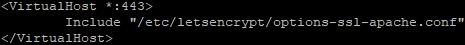
\includegraphics[scale=1.0]{images/apache_config_edit_example.png}
\caption{A kiragadott példakód által generált konfiguráció}
\label{fig:newly_inserted_apache_block}
\end{figure}

\Section{Modulok használata Lua-ban}

Az összes modul, továbbá a main.lua-ban található felhasználói interface is különböző modulokat használ fel. Ezeket a modulokat a \texttt{require} funkcióval lehet betölteni. A \texttt{require} funkció működése hasonló a \texttt{dofile} funkcióhoz, azonban két főbb különbség is van köztük. 

Az egyik az, hogy a require funkció egy megadott path-on belül keresi a betöltendő fájlt, a másik pedig, a require funkció nem engedi ugyanazon fájl duplikált betöltését. Tehát ha már egyszer betöltöttünk egy modult, akkor nem tölti be mégegyszer teljesen, hanem elcachezi egy táblában a már betöltött fájlt. Ha azonban több virtuális path-ot (például: \texttt{\detokenize{?;?.lua}} foo.lua helyett), nevet használunk ugyanazon fájlra, akkor többször is betöltődnek, mivel más lesz a fájl neve, viszont a tartalom ugyan az marad. \cite{require}

A program kódjában a main.lua-ban van megadva, hogy milyen megadott path mentén keresi meg az adott betöltendő fájlt:

\begin{lua}
package.path = package.path..";modules/?.lua";
\end{lua}

Ez a sor szimplán hozzáfűzi a package-k betöltésének pathjához a modules mappát.

Emiatt lehetséges az, hogy nem kell a .lua extensiont kiírnunk a require meghívásaink végén, továbbá, hogy tudunk modulokat betölteni például így:
\begin{lua}
local OpenVPNHandler = require("vpnHandler/OpenVPN");
local linux = require("linux");
\end{lua}

A require funkció a háttérben a megadott fájl kódját futtatja le. Így működik például a \textit{Client} class implementációja az összes modulban is, amelybe be van töltve a config handler, mivel a Client tábla globális változó. 

Minden fájl egy adott code-scope, azonban a globális változók hozzáférhetőek azokban a modulokban is, amelyek betöltötték az adott modult. Emiatt lehetséges például a lokálisan definiált funkciók, változók szeparációja. Az adott modulok a saját maguk kódjában használják őket, viszont az őt betöltő modulok már nem tudnak hozzáférni ezekhez a funkciókhoz, változókhoz.

Modulok esetében a saját implementációmban egy lokális tábla hozódik létre (tehát alapvetőleg "private" láthatóságú), azonban mégis tudjuk használni azt. Ez azért van, mert a require funkció az adott kód lefutási értékét adja vissza. Így lehet akár funkcióval is visszatérni, ami konstruktorként szolgálhat (és az adja vissza a module belső táblát), vagy lehet akár a module táblával is visszatérni. Ha a module tábla nem lokális változó lenne, a modulok implementációi egymással konfliktusba kerülnének.
\Chapter{Tesztelés}

Az elkészült alkalmazás Lua-ban íródott. Legelőször root jogosultságokhoz kell jussunk, akár az \texttt{su}, vagy a \texttt{sudo} parancs használatával. A program futtatása előtt meg kell győződnünk arról, hogy legalább 5.3-as Lua verzióval rendelkezünk az adott számítógépen. 

Ezt így ellenőrizhetjük:
\begin{verbatim}
# lua -v
Lua 5.4.4  Copyright (C) 1994-2022 Lua.org, PUC-Rio
\end{verbatim}

Ha esetleg nem lenne Lua feltelepítve, akkor a következő paranccsal tehetjük meg Debian/Ubuntu esetén:

\begin{verbatim}
# apt-get install lua5.4
\end{verbatim}

Ezután nincs más dolgunk, mint lefuttatni magát az alkalmazást:

\begin{verbatim}
# lua main.lua
\end{verbatim}

Ha nem rendelkezünk root jogosultságokkal, akkor az alkalmazás hibával tér vissza, ez látható \myaref{fig:root_required} ábrán.

\begin{figure}[h]
\centering
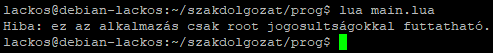
\includegraphics[scale=1]{images/root_required.png}
\caption{root jogosultságok hiányára figyelmeztető hiba}
\label{fig:root_required}
\end{figure}

A program sikeres lefuttatása után a főmenübe érkezünk, amit megtekinthetünk \myaref{fig:main_menu} ábrán.

\begin{figure}[h]
\centering
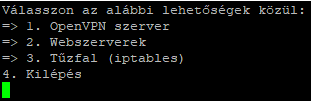
\includegraphics[scale=1]{images/main_menu.png}
\caption{A program főmenüje}
\label{fig:main_menu}
\end{figure}

A program összes menüjében úgy navigálhatunk, hogy beírjuk a sorszámot (például 1, vagy 1.) és ENTER-t nyomunk. A program törekszik arra, hogy minden instrukciót megadjon a felhasználó számára a használatára vonatkozóan. Ha hibába ütközik, kiírja a hiba kódját, továbbá lehetséges forrását.

\pagebreak

\Section{OpenVPN}

Az OpenVPN menüjébe érve \myaref{fig:openvpn_before_install} ábrán látható menüpontok jelennek meg eleinte, ha nincs feltelepítve.

\begin{figure}[h]
\centering
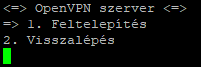
\includegraphics[scale=1]{images/openvpn_install.png}
\caption{OpenVPN főmenü - még feltelepítés előtt}
\label{fig:openvpn_before_install}
\end{figure}

Ekkor csak szimplán kiválasztjuk az egyes menüpontot, és feltelepítődik magától az OpenVPN, ekkor frissülni fog a menü \myaref{fig:openvpn_preconfig} ábrán látható módon.

\begin{figure}[h]
\centering
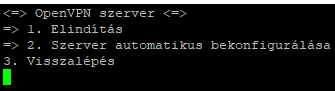
\includegraphics[scale=1]{images/openvpn_preconfig.png}
\caption{OpenVPN főmenü - még konfigurálás előtt}
\label{fig:openvpn_preconfig}
\end{figure}

\SubSection{Konfigurálás, telepítés után}
Konfiguráljuk be a szervert telepítés után. Konfigurálás után a program mappájában létrejön egy openvpn mappa, amely az easyrsa programot tartalmazza. Itt található meg a saját tanusítványkezelőnk (Certificate Authority-nk), amellyel a kliensek és a szerver tanusítványát, privát kulcsát kezeli a program.

Konfigurálás után több menüpont is rendelkezésünkre fog állni, ezeket \myaref{fig:openvpn_after_install} ábrán tudjuk megtekinteni.

\begin{figure}[h]
\centering
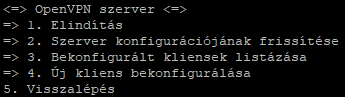
\includegraphics[scale=1]{images/openvpn_after_install.png}
\caption{OpenVPN főmenü - telepítés, konfigurálás után}
\label{fig:openvpn_after_install}
\end{figure}

A 3. menüpontban tudjuk megtekinteni a jelenleg már konfigurált klienseinket, további menüpontok nyílnak onnan: vissza tudjuk vonni egy kliens hozzáférését az OpenVPN szerverhez, továbbá ki tudjuk iratni a kliens konfigját. A kliens konfigja teljesen kimásolható, csak az IP-címet kell átírni benne a saját szerverünk IP-címére. Mindent tartalmaz beágyazva (a certificatet, kulcsfájlokat, tls-crypt fájlt, satöbbit).
Ha egy kliens hozzáférését visszavonjuk, akkor a hozzá generált certificatek, kulcsok revokeolásra kerülnek, és a kliens neve újra felhasználható lesz.

A 4. menüpontban tudunk új klienst létrehozni, két adatot kér be: a kliens nevét, amellyel azonosíthatjuk és egy jelszót a privát kulcsához. A jelszó megadása biztonsági okokból kötelező. A kliens nevének egyedinek kell lennie, duplikáció nem megengedett.

\pagebreak

\Section{Webszerverek}
A webszerverek menüjébe érve választhatunk \textit{Apache} és \textit{nginx} között is. A két webszerver kezelőfelülete között nincs különbség, teljesen egy kódstruktúrára is épülnek, ezért egyben fogom bemutatni őket. Értelemszerűen ha nincs feltelepítve az adott webszerver, akkor \myaref{fig:web_before_install} ábrán látható módon a telepítést fogja felajánlani.

\begin{figure}[h]
\centering
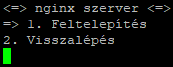
\includegraphics[scale=1]{images/web_before_install.png}
\caption{Webszerver főmenü - telepítés előtt}
\label{fig:web_before_install}
\end{figure}

Telepítés után több menüpont elérhető lesz, ez \myaref{fig:web_after_install} ábrán látható.

\begin{figure}[h]
\centering
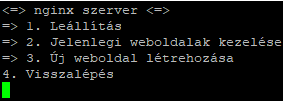
\includegraphics[scale=1]{images/web_after_install.png}
\caption{Webszerver főmenü - telepítés után}
\label{fig:web_after_install}
\end{figure}

A 2. menüpontban tudjuk kezelni a meglévő weboldalainkat, amint kiválasztottunk egyet, utána további menüpontokhoz jutunk:

\begin{itemize}
	\item a legelső menüpont a weboldal törlését jelenti, ez kitörli a weboldal konfigurációját és magát a weboldalt tartalmazó www mappát is,
	\item a második menüpont pedig az SSL certificatek certbot általi generálását szolgálja.
	Több lehetőség is van a certificatek generálására: HTTP-01 challenge, amely egy fájl automatikus elhelyezésével működik; vagy DNS-01 challenge, amelynél a saját névszerverünknél (DNS szerverünknél) beállítások módosítására is szükségünk van. A DNS-01-et akkor célszerű választani, ha valamiért a 80-as portot nem tudjuk használni.
\end{itemize}

A 3. menüpontban tudunk új weboldalakat létrehozni, ehhez magára csak a weboldal címére van szükség. Automatikusan létrehozza a program a weboldal index.html fájlját, a weboldal konfigurációját, továbbá a weboldal www-dirjét, amely \myaref{fig:website_config_dir_examples} látható nginx esetében.

\begin{figure}[h]
\centering
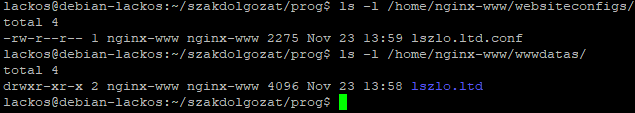
\includegraphics[scale=1]{images/website_config_dir_examples.png}
\caption{Weboldal konfigurációjának helye, weboldal www-dirje nginx esetén}
\label{fig:website_config_dir_examples}
\end{figure}

\pagebreak

\Section{iptables}

Az iptables menüpontot választva, ha nincs még feltelepítve a frontend, akkor felajánlja a program \myaref{fig:iptables_before_install} ábrán látható módon.

\begin{figure}[h]
\centering
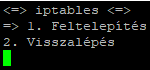
\includegraphics[scale=1]{images/iptables_before_install.png}
\caption{iptables feltelepítése előtt}
\label{fig:iptables_before_install}
\end{figure}

Feltelepítés után több menüpont is a szemünk elé tárul, a menüpontok \myaref{fig:iptables_mainmenu} ábrán tekinthetőek meg.

\begin{figure}[h]
\centering
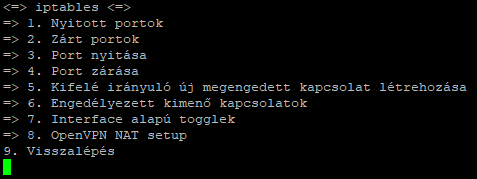
\includegraphics[scale=1]{images/iptables_mainmenu.png}
\caption{iptables főmenüje}
\label{fig:iptables_mainmenu}
\end{figure}

A menüpontok magukért beszélnek. Minden menüpont kiválasztása után felugrik egy interfészt kiválasztó felület, amellyel az adott funkcionalitást leszűkíthetjük egy interfészre. Az interfészválasztás \myaref{fig:iptables_interface_select} ábrán látható.

\begin{figure}[h]
\centering
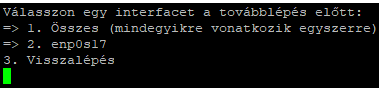
\includegraphics[scale=1]{images/iptables_interface_select.png}
\caption{iptables - interface választása}
\label{fig:iptables_interface_select}
\end{figure}

Ha az összes interfészt választjuk, akkor a program szigorúan azt kezeli, amikor egy szabály ténylegesen mindenre érvényes. Ez azt jelenti iptables esetén, hogy nem adunk meg interfészt hozzá (nem adja hozzá manuálisan a program minden egyes interfacehoz az adott szabályt). Ez azt jelenti, hogy az adott szabály az interfészek változása esetén is megmarad. 

Érdemes ezt figyelembevenni a program használatakor, mert például a nyitott portok lehet, hogy az "all" (vagyis az összes) interfészre vonatkozóan vannak kinyitva, és így nem mutatja ki másik interfészen való nyitott portok lekérdezésekor.

\pagebreak

\texttt{Port nyitáskor} három adatra van szükségünk az interface kiválasztása után: a \textit{protokollra} (tcp/udp/all), a \textit{port számára} és a \textit{bejövő IP-címre}. Ha a bejövő IP-cím üresen marad, bármely IP tud csatlakozni erre a portra.

\texttt{Port záráskor} is három adatra van szükségünk az interface kiválasztása után: a \textit{protokollra} (tcp/udp/all), a \textit{port számára} és a \texttt{bejövő IP-címre}. Ha a bejövő IP-cím üresen marad, mindegyik IP le lesz tiltva erről a portról.

\texttt{Kifelé irányuló új kapcsolat engedélyezésekor} is három adat szükséges: \\a \textit{protokoll} (tcp/udp/all), a \textit{port száma} és a \textit{külső IP-cím}. Ha a port száma üresen marad, akkor a teljes IP-címet engedélyezi kifelé irányuló új kapcsolatként.

A "\texttt{Nyitott portok}", "\texttt{Zárt portok}" és "\texttt{Engedélyezett kimenő kapcsolatok}", továbbá a "\texttt{OpenVPN NAT setup}" menüpont alatt tudjuk ellenőrzni a már meglévő beállításainkat. Ezekben a menüpontokban tudjuk törölni is a már létrehozott szabályokat is.

Az interfész alapú togglek menüpontban van két, a működés szempontjából nagyon fontos beállítás: itt lehet beállítani, hogy minden bejövő, vagy kimenő kapcsolat szűrve legyen-e. Ha egy adott portot kinyitunk, és nem tiltjuk le az összes nem engedélyezett bejövő kapcsolatot, akkor a port nyitás szabály jelenleg épp nem lesz effektív (azonban ígyis megmarad a későbbiekre). Szintén ez vonatkozik a kimenő kapcsolatokra is: ha hozzáadunk egy engedélyezett kimenő kapcsolatot, de nem tiltjuk le a nem engedélyezett kimenő kapcsolatokat, akkor a szabály nem lesz effektív.

Az \texttt{OpenVPN NAT setup} menüpontban tudunk NAT-szabályokat létrehozni az\\ OpenVPN szerverünkhöz, ha feltelepítettük és bekonfiguráltuk a program segítségével. Automatikusan felismeri, ha már van létező NAT szabályunk létrehozva, kilistázza azokat és törölni is tudjuk őket. 

\SubSection{Minden forgalom átirányítása OpenVPN szerveren keresztül}

A NAT bekonfigurálása után, ha minden forgalmat át akarunk irányítani az\\ OpenVPN szerverünkön keresztül a kliens felől, ne felejtsük el a \textit{\detokenize{net.ipv4.ip_forward}} flaget beállítani a Linux szerveren. Továbbá a program alapértelmezésként csak kommentként adja hozzá azt az beállítást az OpenVPN szerver konfigurációjához, amely átirányít minden forgalmat a VPN csatornára, ezt kell kikommentelnünk:

\begin{verbatim}
# nano /etc/openvpn/server_openvpn_serv.conf # ez az alapértelmezett
## elérése az OpenVPN szerver konfigurációnak
\end{verbatim}

Maga a beállítás:
\begin{verbatim}
#push "redirect-gateway def1 bypass-dhcp"
\end{verbatim}

A \detokenize{net.ipv4.ip_forward} flaget pedig a sysctl.conf szerkesztésével tudjuk bekapcsolni:
\begin{verbatim}
# nano /etc/sysctl.conf
# sysctl -p
\end{verbatim}
Ha nincs a flag a fájlban, írjuk bele: "\detokenize{net.ipv4.ip_forward = 1}" ha van, akkor pedig kapcsoljuk be (írjuk át 1-re).



\Chapter{Összefoglalás}

Hasonló szerepe van, mint a bevezetésnek.
Itt már múltidőben lehet beszélni.
A szerző saját meglátása szerint kell összegezni és értékelni a dolgozat fontosabb eredményeit.
Meg lehet benne említeni, hogy mi az ami jobban, mi az ami kevésbé jobban sikerült a tervezettnél.
El lehet benne mondani, hogy milyen további tervek, fejlesztési lehetőségek vannak még a témával kapcsolatban.


\clearpage

\addcontentsline{toc}{chapter}{Irodalomjegyzék}
\bibliographystyle{plain}
\bibliography{dolgozat.bib}

\newpage

\pagestyle{empty}

\noindent \textbf{\Large Adathordozó használati útmutató}

\vskip 1cm

Az adathordozó felépítése egyszerű. Tartalmazza a következő jegyzékeket és fájlokat:
\begin{itemize}
	\item \textbf{latex} jegyzék: Ebben található maga a dolgozat \LaTeX fájljai, benne a fejezetekkel és a mellékletekkel (képekkel).
	\item \textbf{prog} jegyzék: Ez tartalmazza magát a programot. A prog jegyzék felépítése:
		\begin{itemize}
			\item \textbf{\detokenize{openvpn}} jegyzék: Ebben található a saját Certificate Authoritynk (Easy-RSA), ami mind a kliensek, és a szerver certificate \detokenize{&} private key kezeléséért felelős. Runtime hozódik létre, a program használata során.
			\item \textbf{\detokenize{easy_rsa_install_cache}} jegyzék: Runtime hozódik létre, az EasyRSA archívuma található benne.
			\item \textbf{\detokenize{modules}} jegyzék: Itt található maga a program moduljai .lua fájlokban, továbbá ezeken belül is vannak modulokat tartalmazó aljegyzékek.
			\item \textbf{\detokenize{authenticator.lua}} fájl: Certbot használatához szükséges fájl, a DNS-01 challenge implementálásáért felelős.
			\item \textbf{\detokenize{authenticator.sh}} fájl: Egyszerű shell script, amely meghívja az \\\texttt{authenticator.lua} fájlt a Lua interpreterével.
			\item \textbf{\detokenize{main.lua}} fájl: Ez a fájl tartalmazza maga a program kezelőfelületét, továbbá a program implementálása során felmerülő tesztelési kódokat.
		\end{itemize}
	\item \textbf{dolgozat.pdf} fájl: Az elkészült dolgozat PDF formátumban.
\end{itemize}

\end{document}
